% ch12c Superconductivity in metals, part c (书页 233-257 / 分册p045-069)
%--TAIL--
正是由与能隙完全相同的相干因子组合决定的。由此我们立即看出，只要能隙行为良好，$\langle\delta\chi^{2}\rangle$ 在热力学极限下必为零。因此，$\langle b_{\mathbf{p}}\rangle$ 在超导态中取确定值。

\section{准粒子激发}

为了确定往超导体中添加一个额外粒子所需的能量，我们首先求出往 $|\Psi_{\mathrm{BCS}}\rangle$ 中添加一个额外电子的归一化产生算符。一开始我们便注意到
\begin{align*}
a_{\mathbf{p}'\uparrow}^{\dagger}|\Psi_{\mathrm{BCS}}\rangle&=a_{\mathbf{p}'\uparrow}^{\dagger}\prod_{\mathbf{p}}\left(u_{\mathbf{p}}+v_{\mathbf{p}}b_{\mathbf{p}}^{\dagger}\right)|0\rangle\\
&=a_{\mathbf{p}'\uparrow}^{\dagger}u_{\mathbf{p}'}\prod_{\mathbf{p}\neq\mathbf{p}'}\left(u_{\mathbf{p}}+v_{\mathbf{p}}b_{\mathbf{p}}^{\dagger}\right)|0\rangle\\
&=u_{\mathbf{p}'}|\psi_{\mathbf{p}'\uparrow}\rangle\tag{12.217}
\end{align*}
以及
\begin{align*}
a_{-\mathbf{p}'\downarrow}|\Psi_{\mathrm{BCS}}\rangle&=a_{-\mathbf{p}'\downarrow}v_{\mathbf{p}'}a_{\mathbf{p}'\uparrow}^{\dagger}a_{-\mathbf{p}'\downarrow}^{\dagger}\prod_{\mathbf{p}\neq\mathbf{p}'}\left(u_{\mathbf{p}}+v_{\mathbf{p}}b_{\mathbf{p}}^{\dagger}\right)|0\rangle\\
&=-v_{\mathbf{p}'}|\psi_{\mathbf{p}'\uparrow}\rangle,\tag{12.218}
\end{align*}
其中
\begin{equation*}
|\psi_{\mathbf{p}'\uparrow}\rangle=a_{\mathbf{p}'\uparrow}^{\dagger}\prod_{\mathbf{p}\neq\mathbf{p}'}\left(u_{\mathbf{p}}+v_{\mathbf{p}}b_{\mathbf{p}}^{\dagger}\right)|0\rangle\tag{12.219}
\end{equation*}
是在 BCS 基态中添加一个动量为 $\mathbf{p}$、自旋向上的额外电子之后所得的归一化波函数。因此，$a_{\mathbf{p}\uparrow}^{\dagger}$ 与 $a_{-\mathbf{p}\downarrow}$ 并非构造激发态所应使用的算符，因为所得的态未归一化。然而，电子算符的下述线性组合
\begin{equation*}
\gamma_{\mathbf{p}\uparrow}^{\dagger}=u_{\mathbf{p}}^{*}a_{\mathbf{p}\uparrow}^{\dagger}-v_{\mathbf{p}}^{*}a_{-\mathbf{p}\downarrow},\tag{12.220}
\end{equation*}
在作用于 $|\Psi_{\mathrm{BCS}}\rangle$ 时，
\begin{align*}
\gamma_{\mathbf{p}\uparrow}^{\dagger}|\Psi_{\mathrm{BCS}}\rangle&=\left(u_{\mathbf{p}}^{*}a_{\mathbf{p}\uparrow}^{\dagger}-v_{\mathbf{p}}^{*}a_{-\mathbf{p}\downarrow}\right)\prod_{\mathbf{p}'}\left(u_{\mathbf{p}'}+v_{\mathbf{p}'}b_{\mathbf{p}'}^{\dagger}\right)|0\rangle\\
&=\left(|u_{\mathbf{p}}|^{2}+|v_{\mathbf{p}}|^{2}\right)|\psi_{\mathbf{p}\uparrow}\rangle\\
&=|\psi_{\mathbf{p}\uparrow}\rangle\tag{12.221}
\end{align*}
的确产生归一化的态 $|\psi_{\mathbf{p}\uparrow}\rangle$。态 $|\psi_{-\mathbf{p}\downarrow}\rangle$ 相应的产生算符是
\begin{equation*}
\gamma_{-\mathbf{p}\downarrow}^{\dagger}=u_{\mathbf{p}}^{*}a_{-\mathbf{p}\downarrow}^{\dagger}+v_{\mathbf{p}}^{*}a_{\mathbf{p}\uparrow}.\tag{12.222}
\end{equation*}
由于诸 $\gamma_{\mathbf{p}}$ 是诸 $a_{\mathbf{p}}$ 的线性组合，它们必须服从标准的费米–狄拉克反对易关系，即
\begin{align*}
&\left[\gamma_{\mathbf{p}\sigma},\gamma_{\mathbf{p}'\sigma'}^{\dagger}\right]_{+}=\delta_{\mathbf{p}\mathbf{p}'}\delta_{\sigma\sigma'},\\
&\left[\gamma_{\mathbf{p}\sigma},\gamma_{\mathbf{p}'\sigma'}\right]_{+}=\left[\gamma_{\mathbf{p}\sigma}^{\dagger},\gamma_{\mathbf{p}'\sigma'}^{\dagger}\right]_{+}=0.\tag{12.223}
\end{align*}
反对易关系保证
\begin{equation*}
\gamma_{\mathbf{p}\uparrow}|\Psi_{\mathrm{BCS}}\rangle=\gamma_{-\mathbf{p}\downarrow}|\Psi_{\mathrm{BCS}}\rangle=0.\tag{12.224}
\end{equation*}
也就是说，超导体的基态中不存在准粒子。

由于诸 $\gamma_{\mathbf{p}}^{\dagger}$ 是自旋反平行的电子算符与空穴算符的线性组合，由这些算符产生的激发不携带确定的电荷。也就是说，在超导体中产生一个准粒子并不保证电荷守恒。不过，准粒子具有确定的自旋，因为添加一个自旋为 $\hbar/2$ 的电子或一个自旋为 $-\hbar/2$ 的空穴，都会产生 $S_{z}$ 的自旋为 $\hbar/2$ 的本征态。另一方面，库珀对携带电荷 $2e$，但在单态通道中无自旋。因此，在标准的单态 BCS 超导体中，携带确定自旋的量与携带确定电荷的量是彼此不同的实体。正是在这个意义上，单态 BCS 超导体中存在自旋–电荷分离。下面我们证明，单态超导体中自旋载体的能量色散关系是 $\varepsilon_{\mathbf{p}}$。为证明这一论断，我们从 $a_{\mathbf{p}\uparrow}$ 的运动方程出发：
\begin{align*}
\mathrm{i}\hbar\dot{a}_{\mathbf{p}\uparrow}&=\epsilon_{\mathbf{p}}a_{\mathbf{p}\uparrow}-\sum_{\mathbf{p}_{1},\mathbf{p}_{2}}V_{\mathbf{p}_{1}\mathbf{p}_{2}}\left[a_{\mathbf{p}\uparrow},b_{\mathbf{p}_{1}}^{\dagger}b_{\mathbf{p}_{2}}\right]\\
&=\epsilon_{\mathbf{p}}a_{\mathbf{p}\uparrow}+\sum_{\mathbf{p}_{1}}V_{\mathbf{p}\mathbf{p}_{1}}b_{\mathbf{p}_{1}}a_{-\mathbf{p}\downarrow}^{\dagger},\tag{12.225}
\end{align*}
以及 $a_{-\mathbf{p}\downarrow}^{\dagger}$ 的运动方程
\begin{equation*}
\mathrm{i}\hbar\dot{a}_{-\mathbf{p}\downarrow}^{\dagger}=-\epsilon_{\mathbf{p}}a_{-\mathbf{p}\downarrow}^{\dagger}+\sum_{\mathbf{p}_{2}}V_{\mathbf{p}\mathbf{p}_{2}}b_{\mathbf{p}_{2}}^{\dagger}a_{\mathbf{p}\uparrow}.\tag{12.226}
\end{equation*}
为简化这两个运动方程，我们把 $\sum_{\mathbf{p}_{1}}V_{\mathbf{p}\mathbf{p}_{1}}b_{\mathbf{p}_{1}}$ 替换为它的平均值：$-\Delta_{\mathbf{p}}=\sum_{\mathbf{p}_{1}}V_{\mathbf{p}\mathbf{p}_{1}}\langle b_{\mathbf{p}_{1}}\rangle$。于是，有效哈密顿量
\begin{equation*}
H_{\mathrm{eff}}=\sum_{\mathbf{p}\sigma}\epsilon_{\mathbf{p}}n_{\mathbf{p}\sigma}-\sum_{\mathbf{p}}\Delta_{\mathbf{p}}\left(b_{\mathbf{p}}^{\dagger}+b_{\mathbf{p}}\right)\tag{12.227}
\end{equation*}
对配对算符 $b_{\mathbf{p}}^{\dagger}$ 是线性的，不同于完整哈密顿量中的二次型。其结果是，在约化哈密顿量中粒子数不再守恒。尽管如此，BCS 哈密顿量的平均场处理仍然给出超导态的准确描述。这种局面之所以出现，部分原因在于 BCS 基态并不具有固定的粒子数。

平均场闭合导致一组耦合方程：
\begin{align*}
&\mathrm{i}\hbar\dot{a}_{\mathbf{p}\uparrow}=\epsilon_{\mathbf{p}}a_{\mathbf{p}\uparrow}-\Delta_{\mathbf{p}}a_{-\mathbf{p}\downarrow}^{\dagger},\\
&\mathrm{i}\hbar\dot{a}_{-\mathbf{p}\downarrow}^{\dagger}=-\epsilon_{\mathbf{p}}a_{-\mathbf{p}\downarrow}^{\dagger}-\Delta_{\mathbf{p}}a_{\mathbf{p}\uparrow},\tag{12.228}
\end{align*}
它们对能隙参量 $\Delta_{\mathbf{p}}$ 是线性的。为记号简洁，我们把这组方程改写成矩阵形式：
\begin{align*}
\mathrm{i}\hbar\frac{\partial}{\partial t}\begin{pmatrix}a_{\mathbf{p}\uparrow}\\ a_{-\mathbf{p}\downarrow}^{\dagger}\end{pmatrix}&=\begin{pmatrix}\epsilon_{\mathbf{p}} & -\Delta_{\mathbf{p}}\\ -\Delta_{\mathbf{p}} & -\epsilon_{\mathbf{p}}\end{pmatrix}\begin{pmatrix}a_{\mathbf{p}\uparrow}\\ a_{-\mathbf{p}\downarrow}^{\dagger}\end{pmatrix}\\
&=\mathbf{H}_{\mathrm{eff}}\begin{pmatrix}a_{\mathbf{p}\uparrow}\\ a_{-\mathbf{p}\downarrow}^{\dagger}\end{pmatrix}.\tag{12.229}
\end{align*}
为帮助把约化哈密顿量矩阵对角化，我们引入角度 $\theta_{\mathbf{p}}$，使得
\begin{equation*}
\cos\theta_{\mathbf{p}}=\frac{\epsilon_{\mathbf{p}}}{\varepsilon_{\mathbf{p}}}\tag{12.230}
\end{equation*}
以及
\begin{equation*}
\sin\theta_{\mathbf{p}}=\frac{\Delta_{\mathbf{p}}}{\varepsilon_{\mathbf{p}}}.\tag{12.231}
\end{equation*}
这一变换的用处立竿见影，因为 BCS 系数
\begin{equation*}
u_{\mathbf{p}}=\frac{1}{\sqrt{2}}\left(1+\frac{\epsilon_{\mathbf{p}}}{\varepsilon_{\mathbf{p}}}\right)^{1/2}=\frac{1}{\sqrt{2}}\left(1+\cos\theta_{\mathbf{p}}\right)^{1/2}\tag{12.232}
\end{equation*}
与
\begin{equation*}
v_{\mathbf{p}}=\frac{1}{\sqrt{2}}\left(1-\frac{\epsilon_{\mathbf{p}}}{\varepsilon_{\mathbf{p}}}\right)^{1/2}=\frac{1}{\sqrt{2}}\left(1-\cos\theta_{\mathbf{p}}\right)^{1/2}\tag{12.233}
\end{equation*}
构成约化哈密顿量矩阵的本征矢基底，
\begin{equation*}
\mathbf{H}_{\mathrm{eff}}=\varepsilon_{\mathbf{p}}\begin{pmatrix}\cos\theta_{\mathbf{p}} & -\sin\theta_{\mathbf{p}}\\ -\sin\theta_{\mathbf{p}} & -\cos\theta_{\mathbf{p}}\end{pmatrix}.\tag{12.234}
\end{equation*}
该矩阵的本征值是 $\pm 1$。因此，本征矢形如
\begin{equation*}
\begin{pmatrix}\sin\theta_{\mathbf{p}}\\ \cos\theta_{\mathbf{p}}\pm 1\end{pmatrix}.\tag{12.235}
\end{equation*}
本征矢中两组系数之比为
\begin{equation*}
\frac{\sin\theta_{\mathbf{p}}}{(\cos\theta_{\mathbf{p}}\pm 1)}=\pm\left(\tan\frac{\theta_{\mathbf{p}}}{2}\right)^{\pm 1}.\tag{12.236}
\end{equation*}
由于
\begin{equation*}
\tan\frac{\theta_{\mathbf{p}}}{2}=\pm\left(\frac{\sqrt{1-\cos\theta_{\mathbf{p}}}}{\sqrt{1+\cos\theta_{\mathbf{p}}}}\right),\tag{12.237}
\end{equation*}
$\mathbf{H}_{\mathrm{eff}}$ 的本征矢可以写成
\begin{equation*}
\mathbf{e}_{1}=\begin{pmatrix}v_{\mathbf{p}}\\ u_{\mathbf{p}}\end{pmatrix}=\begin{pmatrix}\sin\left(\theta_{\mathbf{p}}/2\right)\\ \cos\left(\theta_{\mathbf{p}}/2\right)\end{pmatrix}\tag{12.238}
\end{equation*}
以及
\begin{equation*}
\mathbf{e}_{2}=\begin{pmatrix}u_{\mathbf{p}}\\ -v_{\mathbf{p}}\end{pmatrix}=\begin{pmatrix}\cos\left(\theta_{\mathbf{p}}/2\right)\\ -\sin\left(\theta_{\mathbf{p}}/2\right)\end{pmatrix}.\tag{12.239}
\end{equation*}
现在可以清楚地看到 $\mathbf{H}_{\mathrm{eff}}\mathbf{e}_{1}=-\varepsilon_{\mathbf{p}}\mathbf{e}_{1}$ 且 $\mathbf{H}_{\mathrm{eff}}\mathbf{e}_{2}=\varepsilon_{\mathbf{p}}\mathbf{e}_{2}$。简言之，$\pm\varepsilon_{\mathbf{p}}$ 是 $\mathbf{H}_{\mathrm{eff}}$ 的两个本征能量。为阐明 $\mathbf{e}_{1}$ 与 $\mathbf{e}_{2}$ 的用处，我们用 $\mathbf{e}_{1}$ 和 $\mathbf{e}_{2}$ 去乘运动方程。对 $\mathbf{e}_{2}$ 的结果
\begin{align*}
\mathrm{i}\hbar\frac{\partial}{\partial t}\left(a_{\mathbf{p}\uparrow}u_{\mathbf{p}}-v_{\mathbf{p}}a_{-\mathbf{p}\downarrow}^{\dagger}\right)&=\mathbf{e}_{2}^{\mathrm{T}}\mathbf{H}_{\mathrm{eff}}\begin{pmatrix}a_{\mathbf{p}\uparrow}\\ a_{-\mathbf{p}\downarrow}^{\dagger}\end{pmatrix}\\
&=\varepsilon_{\mathbf{p}}\mathbf{e}_{2}^{\mathrm{T}}\begin{pmatrix}a_{\mathbf{p}\uparrow}\\ a_{-\mathbf{p}\downarrow}^{\dagger}\end{pmatrix},\tag{12.240}
\end{align*}
表明
\begin{equation*}
\mathrm{i}\hbar\dot{\gamma}_{\mathbf{p}\uparrow}=\varepsilon_{\mathbf{p}}\gamma_{\mathbf{p}\uparrow}.\tag{12.241}
\end{equation*}
类似地，对 $\mathbf{e}_{1}$ 有
\begin{equation*}
\mathrm{i}\hbar\frac{\partial}{\partial t}\left(v_{\mathbf{p}}^{*}a_{\mathbf{p}\uparrow}+u_{\mathbf{p}}^{*}a_{-\mathbf{p}\downarrow}^{\dagger}\right)=-\varepsilon_{\mathbf{p}}\mathbf{e}_{1}^{\dagger}\begin{pmatrix}a_{\mathbf{p}\uparrow}\\ a_{-\mathbf{p}\downarrow}^{\dagger}\end{pmatrix}\tag{12.242}
\end{equation*}
以及
\begin{equation*}
\mathrm{i}\hbar\dot{\gamma}_{-\mathbf{p}\downarrow}^{\dagger}=-\varepsilon_{\mathbf{p}}\gamma_{-\mathbf{p}\downarrow}^{\dagger}.\tag{12.243}
\end{equation*}
这些运动方程意味着约化哈密顿量对角化后的形式为
\begin{equation*}
\mathbf{H}_{\mathrm{eff}}=\sum_{\mathbf{p}}\varepsilon_{\mathbf{p}}\left(\gamma_{\mathbf{p}\uparrow}^{\dagger}\gamma_{\mathbf{p}\uparrow}+\gamma_{-\mathbf{p}\downarrow}^{\dagger}\gamma_{-\mathbf{p}\downarrow}\right).\tag{12.244}
\end{equation*}

\begin{figure}[H]\centering
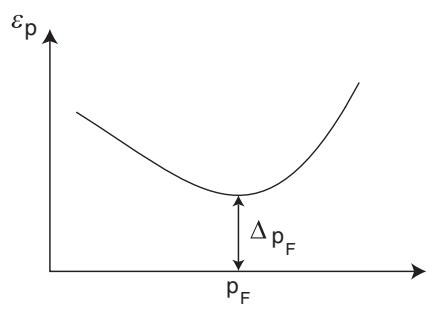
\includegraphics[width=0.44\textwidth]{figs/ch12/fig_12.18_a.jpg}\hfill
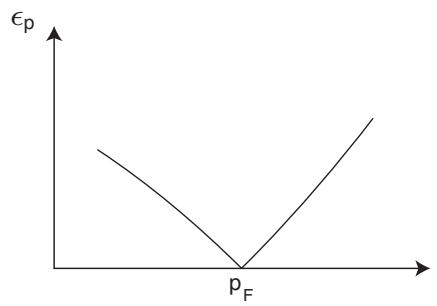
\includegraphics[width=0.44\textwidth]{figs/ch12/fig_12.18_b.jpg}
\caption*{图 12.18\quad (a) 超导态与 (b) 正常态下费米面附近的准粒子谱。$\epsilon_{\mathbf{p}}$ 在费米能级处的取值选定为零。因此，费米面处所需的最小激发能就是能隙能量。}\label{fig:auto:12.18}
\end{figure}

因此，产生任何准粒子，无论其自旋与动量如何，都需要花费能量 $\varepsilon_{\mathbf{p}}$。再强调一遍，BCS 理论的准粒子并不是电子；它们是有自旋但无确定电荷的实体，这与携带电荷 $2e$ 却无自旋的单态库珀对恰成对照。在这个意义上，可以认为 BCS 超导体中存在自旋–电荷分离。准粒子能量的图像示于图 12.18。显然，添加或移除一个粒子至少要花费最小能量 $\Delta_{\mathbf{p}}$。

\section{热力学}

我们现在可以着手计算超导体的热力学性质了。特别有意义的是热容 $C_{\mathrm{v}}$ 与亥姆霍兹自由能，前者在正常态与超导态之间存在不连续。为计算这些量，我们需要把运动方程表述成便于提取有限温度信息的形式。最便捷的做法是用准粒子算符重写模型哈密顿量。为此，我们把准粒子算符反解出来，用它们表示电子算符：
\begin{equation*}
a_{\mathbf{p}\uparrow}=u_{\mathbf{p}}^{*}\gamma_{\mathbf{p}\uparrow}+v_{\mathbf{p}}\gamma_{-\mathbf{p}\downarrow}^{\dagger}\tag{12.245}
\end{equation*}
以及
\begin{equation*}
a_{-\mathbf{p}\downarrow}=-v_{\mathbf{p}}\gamma_{\mathbf{p}\uparrow}^{\dagger}+u_{\mathbf{p}}^{*}\gamma_{-\mathbf{p}\downarrow}.\tag{12.246}
\end{equation*}
我们将证明，热平均
\begin{equation*}
\langle\gamma_{\mathbf{p}\sigma}^{\dagger}\gamma_{\mathbf{p}\sigma}\rangle=n_{\mathbf{p}\sigma},\tag{12.247}
\end{equation*}
其中 $n_{\mathbf{p}\sigma}$ 是在准粒子能量 $\varepsilon_{\mathbf{p}}$ 处取值的费米–狄拉克分布函数。我们将假定与这类准粒子激发相联系的熵由第 2 章给出的无相互作用形式
\begin{equation*}
S=-k_{\mathrm{B}}\sum_{\mathbf{p},\sigma}\left[n_{\mathbf{p}\sigma}\ln n_{\mathbf{p}\sigma}+\left(1-n_{\mathbf{p}\sigma}\right)\ln\left(1-n_{\mathbf{p}\sigma}\right)\right]\tag{12.248}
\end{equation*}
给出。与式 (12.244) 相结合，费米–狄拉克分布便必然成立。尽管如此，我们仍将显式地建立这一结果。

我们先计算亥姆霍兹自由能 $F=E'-TS$，其中 $E'=\langle H-\mu N\rangle$。需要在平均场层次上把内能
\begin{equation*}
E'=\sum_{\mathbf{p},\sigma}\epsilon_{\mathbf{p}}\langle a_{\mathbf{p}\sigma}^{\dagger}a_{\mathbf{p}\sigma}\rangle+\sum_{\mathbf{p},\mathbf{p}'}V_{\mathbf{p}\mathbf{p}'}\langle b_{\mathbf{p}}^{\dagger}\rangle\langle b_{\mathbf{p}'}\rangle,\tag{12.249}
\end{equation*}
用诸 $\gamma_{\mathbf{p}}$ 表示出来。这些表达式中的热平均应理解为对系统所有态的求迹。基态之上的一个任意激发态表示为
\begin{equation*}
|\text{激发态}\rangle=\prod_{i}\gamma_{\mathbf{p}_{i}\sigma_{i}}^{\dagger}|\Psi_{\mathrm{BCS}}\rangle\tag{12.250}
\end{equation*}
因而含有确定数目的被激发准粒子。于是，任何 $\langle\gamma\gamma\rangle$ 形式的平均恒等于零。由式 (12.245) 与式 (12.246) 可得
\begin{align*}
\sum_{\mathbf{p},\sigma}\langle a_{\mathbf{p}\sigma}^{\dagger}a_{\mathbf{p}\sigma}\rangle&=\sum_{\mathbf{p}}\Big\langle\big(u_{\mathbf{p}}\gamma_{\mathbf{p}\uparrow}^{\dagger}+v_{\mathbf{p}}^{*}\gamma_{-\mathbf{p}\downarrow}\big)\big(u_{\mathbf{p}}^{*}\gamma_{\mathbf{p}\uparrow}+v_{\mathbf{p}}\gamma_{-\mathbf{p}\downarrow}^{\dagger}\big)\Big\rangle\\
&\quad+\sum_{\mathbf{p}}\Big\langle\big(-v_{\mathbf{p}}^{*}\gamma_{\mathbf{p}\uparrow}+u_{\mathbf{p}}\gamma_{-\mathbf{p}\downarrow}^{\dagger}\big)\big(-v_{\mathbf{p}}\gamma_{\mathbf{p}\uparrow}^{\dagger}+u_{\mathbf{p}}^{*}\gamma_{-\mathbf{p}\downarrow}\big)\Big\rangle\\
&=\sum_{\mathbf{p}}\left(\left|u_{\mathbf{p}}\right|^{2}-\left|v_{\mathbf{p}}\right|^{2}\right)\left(n_{\mathbf{p}\uparrow}+n_{-\mathbf{p}\downarrow}\right)+2\left|v_{\mathbf{p}}\right|^{2}.\tag{12.251}
\end{align*}
在基态中，我们前面已经证明（见式 (12.171)）$\langle b_{\mathbf{p}}\rangle=u_{\mathbf{p}}^{*}v_{\mathbf{p}}$。有限温度下，配对算符的平均值
\begin{align*}
\langle b_{\mathbf{p}}\rangle&=\langle a_{-\mathbf{p}\downarrow}a_{\mathbf{p}\uparrow}\rangle=\Big\langle\big(-v_{\mathbf{p}}\gamma_{\mathbf{p}\uparrow}^{\dagger}+u_{\mathbf{p}}^{*}\gamma_{-\mathbf{p}\downarrow}\big)\big(u_{\mathbf{p}}^{*}\gamma_{\mathbf{p}\uparrow}+v_{\mathbf{p}}\gamma_{-\mathbf{p}\downarrow}^{\dagger}\big)\Big\rangle\\
&=v_{\mathbf{p}}u_{\mathbf{p}}^{*}\left(1-n_{-\mathbf{p}\downarrow}-n_{\mathbf{p}\uparrow}\right)\tag{12.252}
\end{align*}
包含反映费米能级上下电子配对的热因子。因此，
\begin{equation*}
\sum_{\mathbf{p},\mathbf{p}'}V_{\mathbf{p}\mathbf{p}'}\langle b_{\mathbf{p}}^{\dagger}\rangle\langle b_{\mathbf{p}'}\rangle=\sum_{\mathbf{p},\mathbf{p}'}V_{\mathbf{p}\mathbf{p}'}\,u_{\mathbf{p}}u_{\mathbf{p}'}^{*}v_{\mathbf{p}}^{*}v_{\mathbf{p}'}\left(1-n_{\mathbf{p}\uparrow}-n_{-\mathbf{p}\downarrow}\right)\left(1-n_{-\mathbf{p}'\downarrow}-n_{\mathbf{p}'\uparrow}\right),\tag{12.253}
\end{equation*}
总的亥姆霍兹能量即为
\begin{align*}
F'&=\sum_{\mathbf{p}}\epsilon_{\mathbf{p}}\left[\left(\left|u_{\mathbf{p}}\right|^{2}-\left|v_{\mathbf{p}}\right|^{2}\right)\left(n_{\mathbf{p}\uparrow}+n_{-\mathbf{p}\downarrow}\right)+2\left|v_{\mathbf{p}}\right|^{2}\right]\\
&\quad+\sum_{\mathbf{p},\mathbf{p}'}V_{\mathbf{p}\mathbf{p}'}\left(1-n_{-\mathbf{p}\downarrow}-n_{\mathbf{p}\uparrow}\right)\left(1-n_{-\mathbf{p}'\downarrow}-n_{\mathbf{p}'\uparrow}\right)u_{\mathbf{p}}v_{\mathbf{p}}^{*}u_{\mathbf{p}'}^{*}v_{\mathbf{p}'}\\
&\quad+k_{\mathrm{B}}T\sum_{\mathbf{p},\sigma}\left[n_{\mathbf{p}\sigma}\ln n_{\mathbf{p}\sigma}+\left(1-n_{\mathbf{p}\sigma}\right)\ln\left(1-n_{\mathbf{p}\sigma}\right)\right].\tag{12.254}
\end{align*}
对 $u_{\mathbf{p}}$ 与 $v_{\mathbf{p}}$ 求 $F'$ 的极小，得到标准结果 $u_{\mathbf{p}}=\left(\left(1+\cos\theta_{\mathbf{p}}\right)/2\right)^{1/2}$ 与 $v_{\mathbf{p}}=\left(\left(1-\cos\theta_{\mathbf{p}}\right)/2\right)^{1/2}$，且 $\cos\theta_{\mathbf{p}}=\epsilon_{\mathbf{p}}/\varepsilon_{\mathbf{p}}$。但在这种情形下，能隙通过
\begin{align*}
\Delta_{\mathbf{p}}&=-\sum_{\mathbf{p}'}V_{\mathbf{p}\mathbf{p}'}\langle b_{\mathbf{p}'}\rangle\\
&=-\sum_{\mathbf{p}'}V_{\mathbf{p}\mathbf{p}'}\left(1-n_{\mathbf{p}'\uparrow}-n_{-\mathbf{p}'\downarrow}\right)u_{\mathbf{p}'}^{*}v_{\mathbf{p}'},\tag{12.255}
\end{align*}
依赖于温度，其中 $\sin\theta_{\mathbf{p}}=\Delta_{\mathbf{p}}/\varepsilon_{\mathbf{p}}$。对 $n_{\mathbf{p}\uparrow}$ 变分 $F'$，我们得到
\begin{equation*}
\frac{\partial F'}{\partial n_{\mathbf{p}\uparrow}}=0=\epsilon_{\mathbf{p}}\left(\left|u_{\mathbf{p}}\right|^{2}-\left|v_{\mathbf{p}}\right|^{2}\right)+k_{\mathrm{B}}T\ln\left(\frac{n_{\mathbf{p}\uparrow}}{1-n_{\mathbf{p}\uparrow}}\right)+2\Delta_{\mathbf{p}}u_{\mathbf{p}}v_{\mathbf{p}}^{*},\tag{12.256}
\end{equation*}
其中相干因子 $u_{\mathbf{p}}$ 与 $v_{\mathbf{p}}$ 保持固定。此时加在 $n_{\mathbf{p}\uparrow}$ 上的条件，即
\begin{align*}
k_{\mathrm{B}}T\ln\left(n_{\mathbf{p}\uparrow}^{-1}-1\right)&=\epsilon_{\mathbf{p}}\cos\theta_{\mathbf{p}}+2\Delta_{\mathbf{p}}u_{\mathbf{p}}v_{\mathbf{p}}^{*}\\
&=\epsilon_{\mathbf{p}}\cos\theta_{\mathbf{p}}+\Delta_{\mathbf{p}}\sin\theta_{\mathbf{p}}\\
&=\varepsilon_{\mathbf{p}},\tag{12.257}
\end{align*}
不过是要求 $n_{\mathbf{p}\uparrow}$ 为在准能量 $\varepsilon_{\mathbf{p}}$ 处取值的费米–狄拉克分布。费米–狄拉克分布是有限温度下准粒子激发的最概然分布。

若采用能隙的平均场值，即式 (12.255)，自由能的计算便直截了当：
\begin{align*}
E'&=\sum_{\mathbf{p}}\epsilon_{\mathbf{p}}\left[\left(\left|u_{\mathbf{p}}\right|^{2}-\left|v_{\mathbf{p}}\right|^{2}\right)\left(n_{\mathbf{p}\uparrow}+n_{\mathbf{p}\downarrow}\right)+2\left|v_{\mathbf{p}}\right|^{2}\right]-\sum_{\mathbf{p}}\Delta_{\mathbf{p}}\frac{\sin\theta_{\mathbf{p}}}{2}\left(1-2n_{\mathbf{p}}\right)\\
&=\sum_{\mathbf{p}}\left[2\epsilon_{\mathbf{p}}\left(\cos\theta_{\mathbf{p}}n_{\mathbf{p}}+\sin^{2}\frac{\theta_{\mathbf{p}}}{2}\right)-\Delta_{\mathbf{p}}\frac{\sin\theta_{\mathbf{p}}}{2}\left(1-2n_{\mathbf{p}}\right)\right].\tag{12.258}
\end{align*}
结合 $\ln\left(1/n_{\mathbf{p}\sigma}-1\right)=\varepsilon_{\mathbf{p}}/k_{\mathrm{B}}T$ 这一事实，我们把熵项简化为
\begin{equation*}
TS=-2k_{\mathrm{B}}T\sum_{\mathbf{p}}\left[\beta\varepsilon_{\mathbf{p}}n_{\mathbf{p}}+\ln\left(1+\mathrm{e}^{-\beta\varepsilon_{\mathbf{p}}}\right)\right].\tag{12.259}
\end{equation*}
总自由能即为
\begin{align*}
F'&=\sum_{\mathbf{p}}\left[2\epsilon_{\mathbf{p}}\left(\cos\theta_{\mathbf{p}}n_{\mathbf{p}}+\sin^{2}\frac{\theta_{\mathbf{p}}}{2}\right)-\Delta_{\mathbf{p}}\frac{\sin\theta_{\mathbf{p}}}{2}\left(1-2n_{\mathbf{p}}\right)\right]\\
&\quad+2k_{\mathrm{B}}T\sum_{\mathbf{p}}\left[\beta\varepsilon_{\mathbf{p}}n_{\mathbf{p}}+\ln\left(1+\mathrm{e}^{-\beta\varepsilon_{\mathbf{p}}}\right)\right].\tag{12.260}
\end{align*}
这一表达式的求值留作课后习题（见习题 12.10）。热容
\begin{align*}
C_{\mathrm{v}}&=T\left(\frac{\partial S}{\partial T}\right)_{V}\\
&=-k_{\mathrm{B}}T\sum_{\mathbf{p},\sigma}\frac{\partial n_{\mathbf{p}\sigma}}{\partial T}\ln\left(\frac{n_{\mathbf{p}\sigma}}{1-n_{\mathbf{p}\sigma}}\right)\\
&=\sum_{\mathbf{p},\sigma}\varepsilon_{\mathbf{p}}\frac{\partial n_{\mathbf{p}\sigma}}{\partial T},\tag{12.261}
\end{align*}
包含温度导数
\begin{equation*}
\frac{\partial n_{\mathbf{p}}}{\partial T}=\frac{n_{\mathbf{p}}^{2}}{k_{\mathrm{B}}T}\left[\frac{\varepsilon_{\mathbf{p}}}{T}-\frac{\partial\varepsilon_{\mathbf{p}}}{\partial T}\right]\mathrm{e}^{\beta\varepsilon_{\mathbf{p}}},\tag{12.262}
\end{equation*}
其中又叠加了能隙 $\Delta_{\mathbf{p}}$ 的隐式温度依赖。由 $\varepsilon_{\mathbf{p}}$ 的定义可得
\begin{equation*}
\frac{\partial\varepsilon_{\mathbf{p}}}{\partial T}=\frac{\partial\varepsilon_{\mathbf{p}}}{\partial\Delta_{\mathbf{p}}}\frac{\partial\Delta_{\mathbf{p}}}{\partial T}=\frac{\Delta_{\mathbf{p}}}{\varepsilon_{\mathbf{p}}}\frac{\partial\Delta_{\mathbf{p}}}{\partial T}=\frac{1}{2\varepsilon_{\mathbf{p}}}\frac{\partial\Delta_{\mathbf{p}}^{2}}{\partial T}.\tag{12.263}
\end{equation*}
由于 $\partial\varepsilon_{\mathbf{p}}/\partial T$ 在正常态中为零，我们把 $T=T_{\mathrm{c}}$ 处超导态与正常态热容之差写成
\begin{align*}
\left(C_{\mathrm{v}}^{\mathrm{S}}-C_{\mathrm{v}}^{\mathrm{N}}\right)_{T=T_{\mathrm{c}}}&=-\beta\sum_{\mathbf{p}}n_{\mathbf{p}}^{2}\frac{\partial\Delta_{\mathbf{p}}^{2}}{\partial T}\mathrm{e}^{\beta\varepsilon_{\mathbf{p}}}\\
&=\sum_{\mathbf{p}}\left.\frac{\partial n_{\mathbf{p}}}{\partial\varepsilon_{\mathbf{p}}}\frac{\partial\Delta_{\mathbf{p}}^{2}}{\partial T}\right|_{T=T_{\mathrm{c}}}.\tag{12.264}
\end{align*}
在 $T=T_{\mathrm{c}}$ 附近，能隙很好地近似为 $\Delta^{2}\sim|1-T/T_{\mathrm{c}}|$。于是我们发现 $\partial\Delta^{2}/\partial T\sim 1/T_{\mathrm{c}}$，而热容的不连续严格等于
\begin{equation*}
C_{\mathrm{v}}^{\mathrm{S}}-C_{\mathrm{v}}^{\mathrm{N}}=\frac{N(\epsilon_{\mathrm{F}})}{T_{\mathrm{c}}}\tag{12.265}
\end{equation*}
（在 $T=T_{\mathrm{c}}$ 处）。与这一差值相联系的正号表明，恰在 $T_{\mathrm{c}}$ 下方超导态的热容超过 $C_{\mathrm{v}}^{\mathrm{N}}$。

我们要寻找的第二个结果，是 $C_{\mathrm{v}}^{\mathrm{S}}$ 在 $T_{\mathrm{c}}$ 下方不远处的指数式衰减。为得到这一行为，我们在 $T\to 0$ 的极限下分析式 (12.261)。此极限下 $\partial\Delta_{\mathbf{p}}^{2}/\partial T\to 0$，$n_{\mathbf{p}}\to\mathrm{e}^{-\beta\varepsilon_{\mathbf{p}}}$，热容由下式主导：
\begin{align*}
\lim_{T\to 0}C_{\mathrm{v}}&=2\beta^{2}k_{\mathrm{B}}\sum_{\mathbf{p}}\varepsilon_{\mathbf{p}}^{2}n_{\mathbf{p}}\left(1-n_{\mathbf{p}}\right)\\
&\simeq 2\beta^{2}k_{\mathrm{B}}N(\epsilon_{\mathrm{F}})\Delta^{2}(T=0)\int_{0}^{\infty}\mathrm{d}\epsilon\,\mathrm{e}^{-\beta\sqrt{\Delta^{2}(T=0)+\epsilon^{2}}}\\
&\simeq 2\beta^{2}k_{\mathrm{B}}N(\epsilon_{\mathrm{F}})\Delta_{0}^{2}\mathrm{e}^{-\beta\Delta_{0}}\int_{0}^{\infty}\mathrm{d}\epsilon\,\mathrm{e}^{-\beta\epsilon^{2}/2\Delta_{0}}\\
&=N(\epsilon_{\mathrm{F}})\sqrt{\frac{\pi}{2}}\,k_{\mathrm{B}}\beta^{3/2}\Delta_{0}^{5/2}\mathrm{e}^{-\beta\Delta_{0}},\tag{12.266}
\end{align*}
如前所述，它按指数规律衰减，其中 $\Delta_{0}=\Delta(T=0)$。指数衰减由 $T=0$ 处的能隙主导。在简化导出这一结果的积分时，我们利用了积分在 $\Delta\gg\epsilon$ 时最大这一事实。

\section{实验应用}

BCS 理论的一项关键成功，是声子衰减率这类物理观测量可以十分便捷地计算出来。事实上，正是利用 BCS 理论完成的自旋–晶格弛豫时间计算及其随后的实验证实，才促成了 BCS 理论的广泛接受。本节我们显式地完成其中的三个计算：（1）电磁吸收；（2）超声衰减；（3）自旋–晶格弛豫速率。出现在每个计算中的，是相干因子 $u_{\mathbf{p}}$ 与 $v_{\mathbf{p}}$ 的特定组合。我们将会看到，相干因子的每一种组合都能产生完全不同的物理。物理性质与相干因子如此紧密相连，正是 BCS 配对假设的一个标志。在每个计算中，我们都把相干因子当作实数处理。如前所见，对我们所选的简单模型势，即式 (12.41)，相干因子实际上是实的。

\subsection{电磁吸收}

在 BCS 超导体中，频率低于 $\Delta/\hbar$ 的电磁辐射吸收受到抑制。现在我们拥有了显式导出这一结果的工具。在电磁问题中，微扰项通过把动量替换为 $\mathbf{p}-e\mathbf{A}(\mathbf{r},t)/c$ 得到，其中 $\mathbf{A}(\mathbf{r},t)$ 是矢势。准确到 $\mathbf{A}(\mathbf{r},t)$ 的最低阶，微扰具有 $\mathbf{p}\cdot\mathbf{A}+\mathbf{A}\cdot\mathbf{p}$ 的形式。我们将要求矢势满足横向条件 $\nabla\cdot\mathbf{A}=0$。于是，频率为 $\omega_{\mathbf{q}}$ 的电磁波被吸收时微扰的二次量子化形式为
\begin{equation*}
H_{\mathrm{abs}}=-\frac{e}{mcV}\sum_{\mathbf{p},\sigma}\mathbf{A}\cdot\mathbf{p}\,a_{\mathbf{p}+\mathbf{q}\sigma}^{\dagger}a_{\mathbf{p}\sigma}.\tag{12.267}
\end{equation*}

\begin{figure}[H]\centering
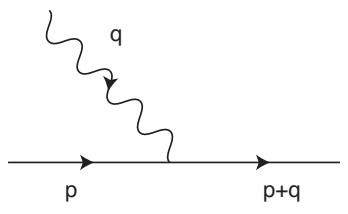
\includegraphics[width=0.44\textwidth]{figs/ch12/fig_12.19_a.jpg}\hfill
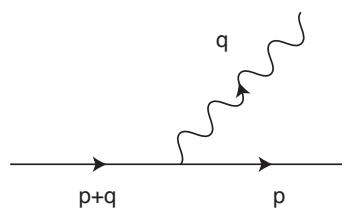
\includegraphics[width=0.44\textwidth]{figs/ch12/fig_12.19_b.jpg}\\[6pt]
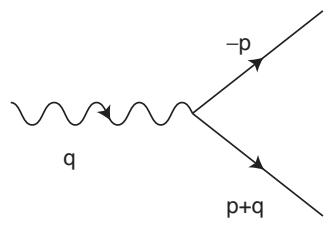
\includegraphics[width=0.5\textwidth]{figs/ch12/fig_12.19_c.jpg}
\caption*{图 12.19\quad 由电磁吸收矩阵元产生的准粒子激发：(a) $\gamma_{\mathbf{p}+\mathbf{q}}^{\dagger}\gamma_{\mathbf{p}}$，(b) $\gamma_{\mathbf{p}}^{\dagger}\gamma_{\mathbf{p}+\mathbf{q}}$，以及 (c) $\gamma_{\mathbf{p}+\mathbf{q}}^{\dagger}\gamma_{-\mathbf{p}}^{\dagger}$。波浪线表示光子相互作用。}\label{fig:auto:12.19}
\end{figure}

我们必须计算形如
\begin{equation*}
\langle f|H_{\mathrm{abs}}|i\rangle=-\frac{e}{mcV}\sum_{\mathbf{p}\sigma}\mathbf{A}\cdot\mathbf{p}\,M_{\mathrm{if}}^{\sigma},\tag{12.268}
\end{equation*}
的矩阵元，其中
\begin{equation*}
M_{\mathrm{if}}^{\sigma}=\langle f|a_{\mathbf{p}+\mathbf{q}\sigma}^{\dagger}a_{\mathbf{p}\sigma}|i\rangle\tag{12.269}
\end{equation*}
而 $|i\rangle$ 与 $|f\rangle$ 分别是初态与末态准粒子态。与热容的计算一样，我们把这个矩阵元
\begin{align*}
\sum_{\sigma}M_{\mathrm{if}}^{\sigma}&=\Big\langle f\Big|\big(u_{\mathbf{p}'}\gamma_{\mathbf{p}'\uparrow}^{\dagger}+v_{\mathbf{p}'}\gamma_{-\mathbf{p}'\downarrow}\big)\big(u_{\mathbf{p}}\gamma_{\mathbf{p}\uparrow}+v_{\mathbf{p}}\gamma_{-\mathbf{p}\downarrow}^{\dagger}\big)\Big|i\Big\rangle\\
&\quad+\Big\langle f\Big|\big(-v_{-\mathbf{p}'}\gamma_{-\mathbf{p}'\uparrow}+u_{-\mathbf{p}'}\gamma_{\mathbf{p}'\downarrow}^{\dagger}\big)\big(-v_{-\mathbf{p}}\gamma_{-\mathbf{p}\uparrow}^{\dagger}+u_{-\mathbf{p}}\gamma_{\mathbf{p}\downarrow}\big)\Big|i\Big\rangle,
\end{align*}
用准粒子算符改写。由上式产生若干种不同的准粒子激发，它们绘于图 12.19 中。

$T=0$ 时基态中没有准粒子。因此，图 12.19 所示的最后一个过程——即产生两个准粒子的过程——是 $T=0$ 下唯一存活的过程。我们就专门考虑 $T=0$ 的情形，因为此时本质物理最易揭示。我们得到
\begin{equation*}
M_{\mathrm{if}}^{\uparrow}+M_{\mathrm{if}}^{\downarrow}=u_{\mathbf{p}+\mathbf{q}}v_{\mathbf{p}}\langle f|\gamma_{\mathbf{p}+\mathbf{q}\uparrow}^{\dagger}\gamma_{-\mathbf{p}\downarrow}^{\dagger}|i\rangle-u_{-(\mathbf{p}+\mathbf{q})}v_{-\mathbf{p}}\langle f|\gamma_{\mathbf{p}+\mathbf{q}\downarrow}^{\dagger}\gamma_{-\mathbf{p}\uparrow}^{\dagger}|i\rangle\tag{12.270}
\end{equation*}
以及
\begin{equation*}
\langle f|H_{\mathrm{abs}}|i\rangle=-\frac{e}{mcV}\sum_{\mathbf{p}}(\mathbf{A}\cdot\mathbf{p})\,\langle f|u_{\mathbf{p}+\mathbf{q}}v_{\mathbf{p}}\gamma_{\mathbf{p}+\mathbf{q}\uparrow}^{\dagger}\gamma_{-\mathbf{p}\downarrow}^{\dagger}-u_{-(\mathbf{p}+\mathbf{q})}v_{\mathbf{p}}\gamma_{\mathbf{p}+\mathbf{q}\downarrow}^{\dagger}\gamma_{-\mathbf{p}\uparrow}^{\dagger}|i\rangle.\tag{12.271}
\end{equation*}
为简化此式，注意若把第二项中的动量作平移 $\mathbf{p}\to-(\mathbf{p}+\mathbf{q})$，则 $\mathbf{p}\cdot\mathbf{A}\to-\mathbf{A}\cdot(\mathbf{p}+\mathbf{q})=-\mathbf{A}\cdot\mathbf{p}$。最后一步等式成立，是因为矢势与电磁场横向。我们得到
\begin{equation*}
\langle f|H_{\mathrm{abs}}|i\rangle=\frac{-e}{mcV}\sum_{\mathbf{p}}(\mathbf{A}\cdot\mathbf{p})\left(u_{\mathbf{p}+\mathbf{q}}v_{\mathbf{p}}-u_{\mathbf{p}}v_{\mathbf{p}+\mathbf{q}}\right)\langle f|\gamma_{\mathbf{p}+\mathbf{q}\uparrow}^{\dagger}\gamma_{-\mathbf{p}\downarrow}^{\dagger}|i\rangle.\tag{12.272}
\end{equation*}
在式 (12.272) 的矩阵元中，我们把末态写成 $|f\rangle=|\mathbf{p}'\uparrow,\mathbf{p}''\downarrow\rangle$。准粒子矩阵元约化为
\begin{equation*}
\langle f|\gamma_{\mathbf{p}+\mathbf{q}\uparrow}^{\dagger}\gamma_{-\mathbf{p}\downarrow}^{\dagger}|i\rangle=\delta_{\mathbf{p}'',-\mathbf{p}}\delta_{\mathbf{p}',\mathbf{p}+\mathbf{q}}.\tag{12.273}
\end{equation*}
单位体积的总吸收速率
\begin{equation*}
\Gamma_{\mathrm{s}}=\frac{2\pi}{\hbar}\left(\frac{e}{mcV}\right)^{2}\sum_{\mathbf{p},\mathbf{p}'}(\mathbf{A}\cdot\mathbf{p})^{2}\delta_{\mathbf{p}+\mathbf{p}',\mathbf{q}}\left(u_{\mathbf{p}'}v_{\mathbf{p}}-u_{\mathbf{p}}v_{\mathbf{p}'}\right)^{2}\delta\left(\varepsilon_{\mathbf{p}}+\varepsilon_{\mathbf{p}'}-\hbar\omega_{\mathbf{q}}\right),\tag{12.274}
\end{equation*}
涉及相干因子
\begin{align*}
\left(u_{\mathbf{p}'}v_{\mathbf{p}}-u_{\mathbf{p}}v_{\mathbf{p}'}\right)^{2}&=\left[\sqrt{\frac{\varepsilon_{\mathbf{p}'}+\epsilon_{\mathbf{p}'}}{2\varepsilon_{\mathbf{p}'}}}\sqrt{\frac{\varepsilon_{\mathbf{p}}-\epsilon_{\mathbf{p}}}{2\varepsilon_{\mathbf{p}}}}-\sqrt{\frac{\varepsilon_{\mathbf{p}'}-\epsilon_{\mathbf{p}'}}{2\varepsilon_{\mathbf{p}'}}}\sqrt{\frac{\varepsilon_{\mathbf{p}}+\epsilon_{\mathbf{p}}}{2\varepsilon_{\mathbf{p}}}}\right]^{2}\\
&=\frac{1}{2\varepsilon_{\mathbf{p}}\varepsilon_{\mathbf{p}'}}\left(\varepsilon_{\mathbf{p}}\varepsilon_{\mathbf{p}'}-\epsilon_{\mathbf{p}}\epsilon_{\mathbf{p}'}-\Delta^{2}\right).\tag{12.275}
\end{align*}
我们把求和化为积分：
\begin{equation*}
\frac{1}{V}\sum_{\mathbf{p}}\to N(\epsilon_{\mathrm{F}})\int\mathrm{d}\epsilon_{\mathbf{p}}\int\frac{\mathrm{d}\Omega_{\mathbf{p}}}{4\pi},\tag{12.276}
\end{equation*}
其中 $\mathrm{d}\Omega_{\mathbf{p}}$ 表示对立体角的积分。吸收速率此时为
\begin{align*}
\Gamma_{\mathrm{s}}&=N(\epsilon_{\mathrm{F}})^{2}\frac{2\pi}{\hbar}\int\mathrm{d}\epsilon\,\mathrm{d}\epsilon'\,\delta\left(\varepsilon+\varepsilon'-\hbar\omega_{\mathbf{q}}\right)\frac{\varepsilon\varepsilon'-\epsilon\epsilon'-\Delta^{2}}{2\varepsilon\varepsilon'}\\
&\quad\times\int\frac{\mathrm{d}\Omega}{4\pi}\frac{\mathrm{d}\Omega'}{4\pi}\,\delta\left(\mathbf{p}+\mathbf{p}'-\mathbf{q}\right)\left(\frac{e}{mc}\mathbf{p}\cdot\mathbf{A}\right)^{2}.\tag{12.277}
\end{align*}
首先注意，围绕费米面的对称性决定了在变换 $\epsilon\leftrightarrow-\epsilon$ 下必须得到相同的结果。因此，$\epsilon\epsilon'$ 项消失。如果我们主要关心费米面附近的贡献，则可令 $|\mathbf{p}|=|\mathbf{p}'|=p_{\mathrm{F}}$。角度项是平凡的，给出 $(p_{\mathrm{F}}Ae)^{2}/3(mc)^{2}$。剩下的积分是
\begin{equation*}
\Gamma_{\mathrm{s}}=N(\epsilon_{\mathrm{F}})^{2}\frac{8\pi}{3\hbar}\left(\frac{p_{\mathrm{F}}Ae}{mc}\right)^{2}\int_{0}^{\infty}\mathrm{d}\epsilon\int_{0}^{\infty}\mathrm{d}\epsilon'\,\delta\left(\varepsilon+\varepsilon'-\hbar\omega_{\mathbf{q}}\right)\frac{\varepsilon\varepsilon'-\Delta^{2}}{2\varepsilon\varepsilon'},\tag{12.278}
\end{equation*}

\begin{figure}[H]\centering
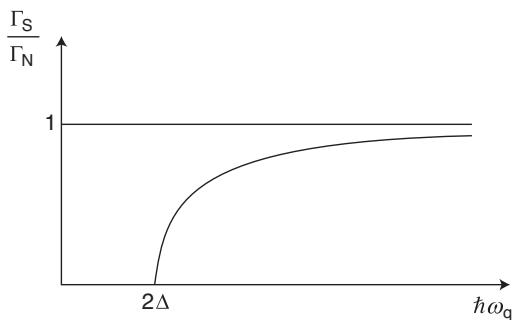
\includegraphics[width=0.55\textwidth]{figs/ch12/fig_12.20.jpg}
\caption*{图 12.20\quad 超导态电磁吸收与正常态电磁吸收之比。横轴为频率，$\Delta$ 为能隙能量。}\label{fig:auto:12.20}
\end{figure}

积分遍及自由粒子能量。因子 4 来自把积分下限从 $-\infty$ 换到零的转换。由于 $\Gamma_{\mathrm{s}}>0$，积分必须对所有的 $\varepsilon$ 与 $\varepsilon'$ 都为正。我们立即看到 $\varepsilon\varepsilon'>\Delta^{2}$，或等价地 $\hbar\omega_{\mathbf{q}}>2\Delta$。因此，当 $\hbar\omega_{\mathbf{q}}<2\Delta$ 时 $\Gamma_{\mathrm{s}}$ 必为零。这就是本节的主要结果。

通过变量替换可以得到更定量的预言。注意由于 $\varepsilon=(\epsilon^{2}+\Delta^{2})^{1/2}$，有 $\varepsilon\,\mathrm{d}\varepsilon=\epsilon\,\mathrm{d}\epsilon$。这一变量替换在 $\varepsilon$ 与 $\varepsilon'$ 的积分范围上引入了一个下限截断：
\begin{equation*}
\Gamma_{\mathrm{s}}=\mathrm{const.}\int_{\Delta}^{\infty}\mathrm{d}\varepsilon\int_{\Delta}^{\infty}\mathrm{d}\varepsilon'\,\delta\left(\varepsilon+\varepsilon'-\hbar\omega_{\mathbf{q}}\right)\frac{\left(\varepsilon\varepsilon'-\Delta^{2}\right)}{\left(\varepsilon^{\prime 2}-\Delta^{2}\right)^{1/2}\left(\varepsilon^{2}-\Delta^{2}\right)^{1/2}}\tag{12.279}
\end{equation*}
$\delta$ 函数约束 $\varepsilon'-\hbar\omega_{\mathbf{q}}=-\varepsilon$ 使我们能把 $\varepsilon$ 积分改写为
\begin{equation*}
\Gamma_{\mathrm{s}}=\mathrm{const.}\int_{\Delta}^{\hbar\omega_{\mathbf{q}}-\Delta}\mathrm{d}\varepsilon\,\frac{\varepsilon\left(\hbar\omega_{\mathbf{q}}-\varepsilon\right)-\Delta^{2}}{\left(\varepsilon^{2}-\Delta^{2}\right)^{1/2}\left(\left(\hbar\omega_{\mathbf{q}}-\varepsilon\right)^{2}-\Delta^{2}\right)^{1/2}},\tag{12.280}
\end{equation*}
其中我们把积分上限近似取为下界 $\hbar\omega_{\mathbf{q}}-\Delta$。当 $\Delta=0$ 时，被积函数化为常数，$\Gamma_{\mathrm{s}}\to\mathrm{const.}\,\hbar\omega_{\mathbf{q}}$。若把 $\Gamma_{\mathrm{s}}$ 的 $\Delta=0$ 值记为 $\Gamma_{\mathrm{N}}$ 并绘出 $\Gamma_{\mathrm{s}}/\Gamma_{\mathrm{N}}$，便得到图 12.20 所示的结果。我们在此导出的 $\Gamma_{\mathrm{s}}$ 形式与实验符合得很好。

\subsection{超声衰减}

现在考虑一束声子入射到超导体上的问题。我们曾经预告，除非入射声子束的能量超过 $2\Delta$，超导体对声子吸收应当是透明的。为证明这一点，我们用准粒子算符重写电子–声子哈密顿量，即式 (12.23)：
\begin{align*}
H_{\mathrm{e}\text{-}\mathrm{ph}}=\sum_{\mathbf{p},\mathbf{q}}^{\prime}M_{\mathbf{q}}\left(b_{\mathbf{q}}+b_{-\mathbf{q}}^{\dagger}\right)\Big[\big(u_{\mathbf{p}+\mathbf{q}}\gamma_{\mathbf{p}+\mathbf{q}\uparrow}^{\dagger}+v_{\mathbf{p}+\mathbf{q}}\gamma_{-(\mathbf{p}+\mathbf{q})\downarrow}\big)\big(u_{\mathbf{p}}\gamma_{\mathbf{p}\uparrow}+v_{\mathbf{p}}\gamma_{-\mathbf{p}\downarrow}^{\dagger}\big)\\
+\big(u_{-(\mathbf{p}+\mathbf{q})}\gamma_{\mathbf{p}+\mathbf{q}\downarrow}^{\dagger}-v_{-(\mathbf{p}+\mathbf{q})}\gamma_{-(\mathbf{p}+\mathbf{q})\uparrow}\big)\big(u_{-\mathbf{p}}\gamma_{\mathbf{p}\downarrow}-v_{-\mathbf{p}}\gamma_{-\mathbf{p}\uparrow}^{\dagger}\big)\Big],\tag{12.281}
\end{align*}
其中用到式 (12.245) 与式 (12.246)。准粒子–声子耦合产生两类不同的项：（1）单准粒子激发；（2）准粒子对的产生与湮没。单准粒子的产生与湮没过程
\begin{align*}
H_{\mathrm{e}\text{-}\mathrm{ph}}^{\mathrm{qp}}=\sum_{\mathbf{p},\mathbf{q}}^{\prime}M_{\mathbf{q}}\left(b_{\mathbf{q}}+b_{-\mathbf{q}}^{\dagger}\right)\Big[u_{\mathbf{p}+\mathbf{q}}u_{\mathbf{p}}\gamma_{\mathbf{p}+\mathbf{q}\uparrow}^{\dagger}\gamma_{\mathbf{p}\uparrow}+v_{\mathbf{p}+\mathbf{q}}v_{\mathbf{p}}\gamma_{-(\mathbf{p}+\mathbf{q})\downarrow}\gamma_{-\mathbf{p}\downarrow}^{\dagger}\\
+u_{-(\mathbf{p}+\mathbf{q})}u_{-\mathbf{p}}\gamma_{\mathbf{p}+\mathbf{q}\downarrow}^{\dagger}\gamma_{\mathbf{p}\downarrow}+v_{-(\mathbf{p}+\mathbf{q})}v_{-\mathbf{p}}\gamma_{-(\mathbf{p}+\mathbf{q})\uparrow}\gamma_{-\mathbf{p}\uparrow}^{\dagger}\Big],\tag{12.282}
\end{align*}
来自共轭的 $\gamma_{\mathbf{p}},\gamma_{\mathbf{p}'}^{\dagger}$ 对。附加的散射通道
\begin{align*}
H_{\mathrm{e}\text{-}\mathrm{ph}}^{\mathrm{pair}}=\sum_{\mathbf{p},\mathbf{q}}M_{\mathbf{q}}\left(b_{\mathbf{q}}+b_{-\mathbf{q}}^{\dagger}\right)\big[u_{\mathbf{p}+\mathbf{q}}v_{\mathbf{p}}\gamma_{\mathbf{p}+\mathbf{q}\uparrow}^{\dagger}\gamma_{-\mathbf{p}\downarrow}^{\dagger}-u_{-(\mathbf{p}+\mathbf{q})}v_{-\mathbf{p}}\gamma_{\mathbf{p}+\mathbf{q}\downarrow}^{\dagger}\gamma_{-\mathbf{p}\uparrow}^{\dagger}\\
+v_{\mathbf{p}+\mathbf{q}}u_{\mathbf{p}}\gamma_{-(\mathbf{p}+\mathbf{q})\downarrow}\gamma_{\mathbf{p}\uparrow}-v_{-(\mathbf{p}+\mathbf{q})}u_{-\mathbf{p}}\gamma_{-(\mathbf{p}+\mathbf{q})\uparrow}\gamma_{\mathbf{p}\downarrow}\big],\tag{12.283}
\end{align*}
则由准粒子对的产生与湮没来传递。

声子在超导体中被激发时，预期两类过程都会发生。然而，与电磁吸收问题一样，对的产生与湮没预期仅在 $\hbar\omega_{\mathbf{q}}>2\Delta$ 时出现。因为我们的目标是证明频率低于 $2\Delta$ 时声子吸收受到衰减，所以可以忽略配对散射项。于是我们专门考虑 $\hbar\omega_{\mathbf{q}}<\Delta$ 的情形，此时只有单粒子散射对跃迁振幅有贡献。发射项与吸收项的两种代表性类别示于图 12.21(a) 与 12.21(b)。每一项对 $\downarrow$ 与 $\uparrow$ 电子态的贡献相同。先考虑发射。描写单准粒子交换中声子发射的算符是
\begin{equation*}
V_{\mathrm{emiss}}^{\mathrm{qp}}=M_{\mathbf{q}}b_{-\mathbf{q}}^{\dagger}\left(u_{\mathbf{p}+\mathbf{q}}u_{\mathbf{p}}\gamma_{\mathbf{p}+\mathbf{q}\sigma}^{\dagger}\gamma_{\mathbf{p}\sigma}+v_{-(\mathbf{p}+\mathbf{q})}v_{-\mathbf{p}}\gamma_{\mathbf{p}\sigma}\gamma_{\mathbf{p}+\mathbf{q}\sigma}^{\dagger}\right),\tag{12.284}
\end{equation*}
其中我们在式 (12.282) 的第二项中作了 $-\mathbf{p}\to\mathbf{p}$ 与 $-\mathbf{p}-\mathbf{q}\to\mathbf{p}$ 的替换。利用诸 $\gamma$ 的反对易关系，可以把发射项改写为
\begin{equation*}
V_{\mathrm{emiss}}^{\mathrm{qp}}=M_{\mathbf{q}}b_{-\mathbf{q}}^{\dagger}\left[\left(u_{\mathbf{p}+\mathbf{q}}u_{\mathbf{p}}-v_{-(\mathbf{p}+\mathbf{q})}v_{-\mathbf{p}}\right)\gamma_{\mathbf{p}+\mathbf{q}\sigma}^{\dagger}\gamma_{\mathbf{p}\sigma}+v_{-(\mathbf{p}+\mathbf{q})}v_{-\mathbf{p}}\delta_{\mathbf{p},\mathbf{p}+\mathbf{q}}\right].\tag{12.285}
\end{equation*}
最后一项要求 $\mathbf{p}=\mathbf{p}+\mathbf{q}$，等价地 $\mathbf{q}=0$。然而 $M_{\mathbf{q}}$ 线性于 $\mathbf{q}$，故在 $\mathbf{q}=0$ 时为零。在发射过程中，末态的复合电子–声子态必须包含动量为 $\mathbf{q}$ 的声子以及动量为 $\mathbf{p}+\mathbf{q}$、自旋为 $\sigma$ 的准粒子。动量为 $\mathbf{p}$ 的准粒子不出现在这个态中。

\begin{figure}[H]\centering
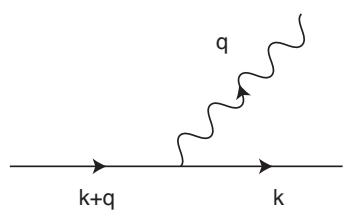
\includegraphics[width=0.42\textwidth]{figs/ch12/fig_12.21_a.jpg}\hfill
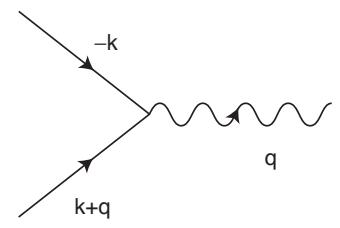
\includegraphics[width=0.4\textwidth]{figs/ch12/fig_12.21_b.jpg}\\[8pt]
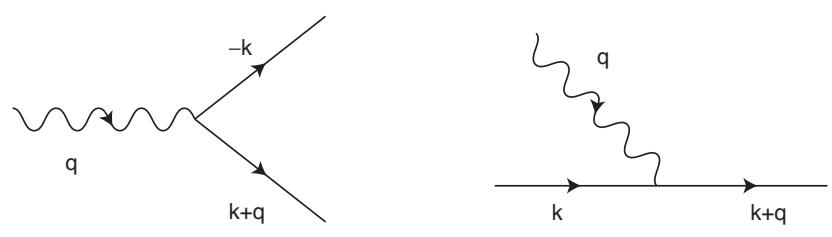
\includegraphics[width=0.82\textwidth]{figs/ch12/fig_12.21_c.jpg}
\caption*{图 12.21\quad 对超声衰减有贡献的 (a) 发射过程与 (b) 吸收过程。波浪线表示准粒子–声子相互作用。}\label{fig:auto:12.21}
\end{figure}

初态一般是包含任意数目准粒子（特别是动量为 $\mathbf{p}$、自旋为 $\sigma$ 的准粒子）的某个行列式态。令 $|\mathbf{p}+\mathbf{q}\sigma,\mathbf{q}\rangle$ 与 $|\mathbf{p}\sigma\rangle$ 分别为末态与初态。发射矩阵元简化为
\begin{equation*}
\langle\mathbf{p}+\mathbf{q}\sigma,\mathbf{q}|V_{\mathrm{emiss}}^{\mathrm{qp}}|\mathbf{p}\sigma\rangle=M_{\mathbf{q}}\left(u_{\mathbf{p}+\mathbf{q}}u_{\mathbf{p}}-v_{-(\mathbf{p}+\mathbf{q})}v_{-\mathbf{p}}\right)\sqrt{N_{\mathbf{q}}+1}\sqrt{n_{\mathbf{p}}\left(1-n_{\mathbf{p}+\mathbf{q}}\right)},\tag{12.286}
\end{equation*}
其中 $n_{\mathbf{p}}$ 是动量态 $\mathbf{p}$ 中准粒子的占据数。于是，同时计入 $\uparrow$ 与 $\downarrow$ 两种自旋后，发射的费米黄金规则速率为
\begin{align*}
\Gamma_{\mathrm{emiss}}^{\mathrm{qp}}&=\frac{2}{\hbar}\sum_{\mathbf{p}}\left(N_{\mathbf{q}}+1\right)\left|M_{\mathbf{q}}\right|^{2}\left(u_{\mathbf{p}+\mathbf{q}}u_{\mathbf{p}}-v_{\mathbf{p}+\mathbf{q}}v_{\mathbf{p}}\right)^{2}\\
&\quad\times n_{\mathbf{p}}\left(1-n_{\mathbf{p}+\mathbf{q}}\right)2\pi\delta\left(\hbar\omega_{\mathbf{q}}+\varepsilon_{\mathbf{p}}-\varepsilon_{\mathbf{p}+\mathbf{q}}\right).\tag{12.287}
\end{align*}
类似的论证可以应用于声子的吸收。跃迁速率的形式有两个主要差异。其一，因子 $N_{\mathbf{q}}+1$ 被换成 $N_{\mathbf{q}}$；这一变化源于吸收情形下末态少一个声子。其二，初态与末态分别形如 $|\mathbf{p}\sigma,\mathbf{q}\rangle$ 与 $|\mathbf{p}+\mathbf{q}\sigma\rangle$。所有这类初、末态之间的吸收速率
\begin{equation*}
\Gamma_{\mathrm{abs}}^{\mathrm{qp}}=\frac{2}{\hbar}\sum_{\mathbf{q}}N_{\mathbf{q}}|M_{\mathbf{q}}|\left(u_{\mathbf{p}+\mathbf{q}}u_{\mathbf{p}}-v_{\mathbf{p}+\mathbf{q}}v_{\mathbf{p}}\right)^{2}n_{\mathbf{p}+\mathbf{q}}\left(1-n_{\mathbf{p}}\right)2\pi\delta\left(\hbar\omega_{\mathbf{q}}+\varepsilon_{\mathbf{p}}-\varepsilon_{\mathbf{p}+\mathbf{q}}\right),\tag{12.288}
\end{equation*}
是各个速率之和，我们在费米黄金规则的层次上处理。

发射速率与吸收速率之差
\begin{align*}
\Gamma_{\mathbf{q}}&=\Gamma_{\mathrm{abs}}^{\mathrm{qp}}-\Gamma_{\mathrm{emiss}}^{\mathrm{qp}}\\
&=\frac{2}{\hbar}\sum_{\mathbf{p}}^{\prime}\left|M_{\mathbf{q}}\right|^{2}\left(u_{\mathbf{p}+\mathbf{q}}u_{\mathbf{p}}-v_{\mathbf{p}+\mathbf{q}}v_{\mathbf{p}}\right)^{2}2\pi\delta\left(\hbar\omega_{\mathbf{q}}+\varepsilon_{\mathbf{p}}-\varepsilon_{\mathbf{p}+\mathbf{q}}\right)\\
&\quad\times\left[N_{\mathbf{q}}\left(n_{\mathbf{p}+\mathbf{q}}-n_{\mathbf{p}}\right)-n_{\mathbf{p}}\left(1-n_{\mathbf{p}+\mathbf{q}}\right)\right],\tag{12.289}
\end{align*}
包含一个通过 $N_{\mathbf{q}}$ 依赖于声子占据的部分和一个不依赖的部分。在合并吸收项与发射项时，我们利用了相干因子的时间反演不变性。不依赖声子占据的部分定义了有效自发发射速率，而第一项定义了 $N_{\mathbf{q}}$ 个声子被吸收的总速率。于是我们定义
\begin{align*}
\frac{\mathrm{d}N_{\mathbf{q}}}{\mathrm{d}t}&=-\frac{2}{\hbar}\sum_{\mathbf{p}}\left|M_{\mathbf{q}}\right|^{2}\left(u_{\mathbf{p}+\mathbf{q}}u_{\mathbf{p}}-v_{\mathbf{p}+\mathbf{q}}v_{\mathbf{p}}\right)^{2}2\pi\delta\left(\hbar\omega_{\mathbf{q}}+\varepsilon_{\mathbf{p}}-\varepsilon_{\mathbf{p}+\mathbf{q}}\right)N_{\mathbf{q}}\left(n_{\mathbf{p}+\mathbf{q}}-n_{\mathbf{p}}\right)\\
&=-\alpha_{\mathbf{q}}N_{\mathbf{q}}\tag{12.290}
\end{align*}
为净声学衰减速率。

为求出 $\alpha_{\mathbf{q}}$，我们把求和化为积分
\begin{align*}
\alpha_{\mathbf{q}}&=\frac{4\pi}{\hbar}\left|M_{\mathbf{q}}\right|^{2}g^{2}(0)\int\mathrm{d}\epsilon_{\mathbf{p}}\,\mathrm{d}\epsilon_{\mathbf{p}'}\left(u_{\mathbf{p}}u_{\mathbf{p}'}-v_{\mathbf{p}}v_{\mathbf{p}'}\right)\left(n_{\mathbf{p}'}-n_{\mathbf{p}}\right)\\
&\quad\times\delta\left(\hbar\omega_{\mathbf{q}}+\varepsilon_{\mathbf{p}}-\varepsilon_{\mathbf{p}'}\right)\int\frac{\mathrm{d}\Omega_{\mathbf{p}}}{4\pi}\frac{\mathrm{d}\Omega_{\mathbf{p}'}}{4\pi}\,\delta\left(\mathbf{p}-\mathbf{p}'-\mathbf{q}\right)\tag{12.291}
\end{align*}
其中动量守恒由角度因子 $\delta\left(\mathbf{p}-\mathbf{p}'-\mathbf{q}\right)$ 保证。为简化式 (12.291)，注意角度因子在正常态与超导态中是相同的。由于假定能隙各向同性，可以把角度依赖分离出来；记该因子为 $A_{\Omega}$。现在我们需要相干因子的表达式：
\begin{equation*}
\left(u_{\mathbf{p}}u_{\mathbf{p}'}-v_{\mathbf{p}}v_{\mathbf{p}'}\right)^{2}=\frac{1}{2\varepsilon_{\mathbf{p}}\varepsilon_{\mathbf{p}'}}\left[\varepsilon_{\mathbf{p}}\varepsilon_{\mathbf{p}'}+\epsilon_{\mathbf{p}}\epsilon_{\mathbf{p}'}-\Delta^{2}\right],\tag{12.292}
\end{equation*}
其中已假定能隙为常数，$\Delta=\Delta_{\mathbf{p}}=\Delta_{\mathbf{p}'}$。注意 $n_{\mathbf{p}}$ 与 $\varepsilon_{\mathbf{p}}$ 都是 $\epsilon_{\mathbf{p}}$ 的偶函数。因此，对线性因子 $\epsilon_{\mathbf{p}}\epsilon_{\mathbf{p}'}$ 的积分因积分限为偶而消失。作为进一步的简化，注意到 $\mathrm{d}\varepsilon_{\mathbf{p}}/\mathrm{d}\epsilon_{\mathbf{p}}=\varepsilon_{\mathbf{p}}/\epsilon_{\mathbf{p}}$，我们把积分变量从 $\epsilon_{\mathbf{p}}$ 换成 $\varepsilon_{\mathbf{p}}$。剩下
\begin{align*}
\alpha_{\mathbf{q}}&=\frac{8\pi}{\hbar}\left|M_{\mathbf{q}}\right|^{2}g^{2}(0)A_{\Omega}\int_{\Delta}^{\infty}\mathrm{d}\varepsilon_{\mathbf{p}}\int_{\Delta}^{\infty}\mathrm{d}\varepsilon_{\mathbf{p}'}\,\frac{\varepsilon_{\mathbf{p}}\varepsilon_{\mathbf{p}'}}{\epsilon_{\mathbf{p}}\epsilon_{\mathbf{p}'}}\left(1-\frac{\Delta^{2}}{\varepsilon_{\mathbf{p}}\varepsilon_{\mathbf{p}'}}\right)\\
&\quad\times\left(n_{\mathbf{p}'}-n_{\mathbf{p}}\right)\delta\left(\hbar\omega_{\mathbf{q}}+\varepsilon_{\mathbf{p}}-\varepsilon_{\mathbf{p}'}\right).\tag{12.293}
\end{align*}
量 $N(0)\,\mathrm{d}\epsilon_{\mathbf{p}}/\mathrm{d}\varepsilon_{\mathbf{p}}=N(0)\varepsilon_{\mathbf{p}}/\epsilon_{\mathbf{p}}$ 大致就是准粒子激发的态密度。在费米面上，$\epsilon_{\mathbf{p}}\to 0$，$\mathrm{d}\epsilon_{\mathbf{p}}/\mathrm{d}\varepsilon_{\mathbf{p}}\to\infty$。但在积分范围内，$\varepsilon_{\mathbf{p}}/\epsilon_{\mathbf{p}}$ 是有限的。在 $\hbar\omega_{\mathbf{q}}\ll\Delta$ 的极限下，$\varepsilon_{\mathbf{p}'}\approx\varepsilon_{\mathbf{p}}$。因此，
\begin{equation*}
\frac{\varepsilon_{\mathbf{p}}}{\epsilon_{\mathbf{p}}}\frac{\varepsilon_{\mathbf{p}'}}{\epsilon_{\mathbf{p}'}}\left(1-\frac{\Delta^{2}}{\varepsilon_{\mathbf{p}}\varepsilon_{\mathbf{p}'}}\right)\to\frac{\varepsilon_{\mathbf{p}}^{2}}{\epsilon_{\mathbf{p}}^{2}}\left(\frac{\varepsilon_{\mathbf{p}}^{2}-\Delta^{2}}{\varepsilon_{\mathbf{p}}^{2}}\right)=1.\tag{12.294}
\end{equation*}

\begin{figure}[H]\centering
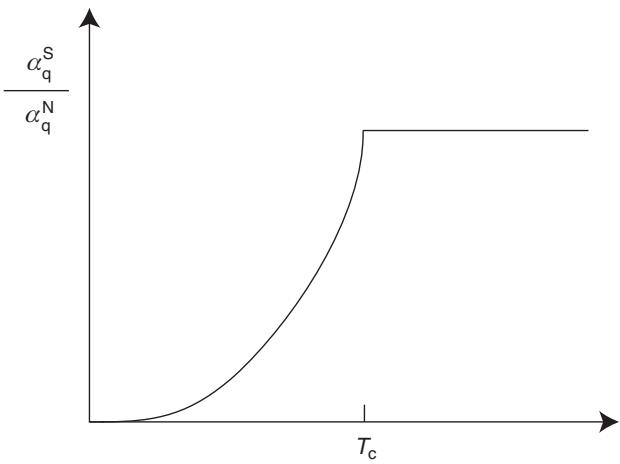
\includegraphics[width=0.55\textwidth]{figs/ch12/fig_12.22.jpg}
\caption*{图 12.22\quad 式 (12.297) 预言的超导态与正常态超声衰减之比。该比值在超导态中的下降是库珀对形成的一个标志。}\label{fig:auto:12.22}
\end{figure}

在这个极限下工作是完全合理的，因为我们考虑的只是单准粒子激发导致的声子吸收。在被积函数中取 $\varepsilon_{\mathbf{p}'}=\varepsilon_{\mathbf{p}}+\hbar\omega_{\mathbf{q}}$，我们得到
\begin{align*}
\alpha_{\mathbf{q}}&=\frac{8\pi}{\hbar}\left|M_{\mathbf{q}}\right|^{2}g^{2}(0)A_{\Omega}\int_{\Delta}^{\infty}\mathrm{d}\varepsilon_{\mathbf{p}}\left(n\left(\varepsilon_{\mathbf{p}}+\hbar\omega_{\mathbf{q}}\right)-n\left(\varepsilon_{\mathbf{p}}\right)\right)\\
&\simeq-\frac{8\pi}{\hbar}\left|M_{\mathbf{q}}\right|^{2}g^{2}(0)A_{\Omega}\hbar\omega_{\mathbf{q}}n(\Delta).\tag{12.295}
\end{align*}
正常态中 $\Delta=0$，于是
\begin{equation*}
\alpha_{\mathbf{q}}^{\mathrm{N}}=-\frac{8\pi}{\hbar}\left|M_{\mathbf{q}}\right|^{2}g^{2}(0)A_{\Omega}\hbar\omega_{\mathbf{q}}n(0)=-\frac{4\pi}{\hbar}\left|M_{\mathbf{q}}\right|^{2}g^{2}(0)A_{\Omega}\hbar\omega_{\mathbf{q}}.\tag{12.296}
\end{equation*}
比值 $\alpha_{\mathbf{q}}^{\mathrm{s}}/\alpha_{\mathbf{q}}^{\mathrm{N}}$ 约化为
\begin{equation*}
\frac{\alpha_{\mathbf{q}}^{\mathrm{s}}}{\alpha_{\mathbf{q}}^{\mathrm{N}}}=\frac{2}{\mathrm{e}^{\beta\Delta(T)}+1}.\tag{12.297}
\end{equation*}
$T=T_{\mathrm{c}}$ 时 $\Delta=0$，该比值给出 1，如图 12.22 所示。超声衰减率的这一计算（文献 [S1964]）与实验结果符合得极好。这里我们再次看到，最终决定超导态中声波吸收的仍然是能隙。当然，这一计算只对纵声子有效。在纵波情形中，$M_{\mathbf{q}}$ 在正常态与超导态中是相同的；而对于横声子，$M_{\mathbf{q}}$ 从正常态到超导态会发生剧烈变化。此时 $M_{\mathbf{q}}$ 的磁性依赖导致 $T=T_{\mathrm{c}}$ 处衰减率发生不连续的骤降，如图 12.23 所示（文献 [S1964]）。

\begin{figure}[H]\centering
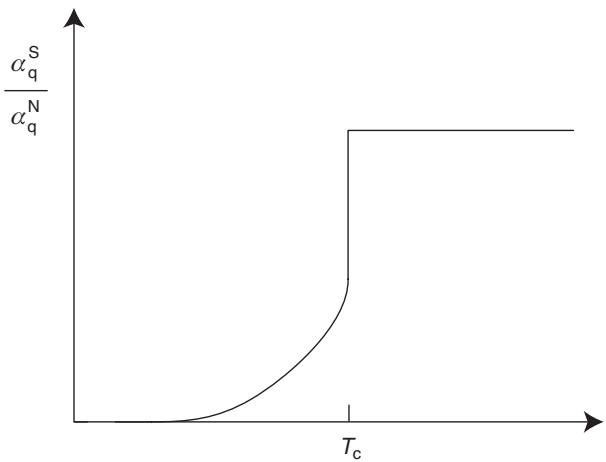
\includegraphics[width=0.55\textwidth]{figs/ch12/fig_12.23.jpg}
\caption*{图 12.23\quad 横声子的超导态与正常态超声吸收速率之比随温度 $T$ 的变化。}\label{fig:auto:12.23}
\end{figure}

\subsection{自旋–晶格弛豫}

我们利用 BCS 相干因子给出的最后一个计算，是自旋–晶格弛豫时间 $T_{1}$ 的计算。出于历史原因，这是一个关键性的计算，因为 $1/T_{1}$ 的峰应出现在 $T_{\mathrm{c}}$ 稍下方，这一预言比 Hebel 与 Slichter 的实验（文献 [HS1959]）更早。事实上，$1/T_{1}$ 在 $T_{\mathrm{c}}$ 稍下方增强的实验证实，是使 BCS 理论获得广泛接受的决定性证据。为定义 $T_{1}$，考虑对一集核自旋施加磁场。磁场撤去之后，自旋将弛豫回去以达到平衡磁化。这一过程所需的时间就称为 $T_{1}$。在绝缘体中，是原子核与电子杂质之间的耦合使核得以弛豫。听其自然，原子核无法达到平衡自旋温度。晶格温度必须由某种媒介传递给原子核。在金属中，提供这一耦合的是传导电子。由于超导体中的电子被锁定在相干态中，我们预期 $T_{1}$ 会被剧烈改变。考虑位于原点 $\mathbf{r}=0$ 处、磁矩为 $\mathbf{S}_{\mathrm{N}}$ 的原子核。$\mathbf{r}=0$ 处的净电子自旋由该处的局域电子自旋密度 $\mathbf{S}=\hbar\Psi^{\dagger}(0)\sigma\Psi(0)/2$ 给出，其中 $\Psi(0)$ 是 $\mathbf{r}=0$ 处的电子波函数，$\sigma$ 是泡利自旋矩阵。费米接触项
\begin{equation*}
H_{\mathrm{int}}=\frac{8\pi}{3}\mu_{\mathrm{B}}\mathbf{S}_{\mathrm{N}}\cdot\mathbf{S},\tag{12.298}
\end{equation*}
定义了 $\mathbf{r}=0$ 处原子核与电子之间的耦合。式 (12.298) 中的 $\mu_{\mathrm{B}}$ 是玻尔磁子。

要把这一耦合用于超导体中 $T_{1}$ 的计算，只需用准粒子算符表示 $\mathbf{S}$。为此，引入旋量场算符
\begin{equation*}
\Psi(\mathbf{r})=\frac{1}{\sqrt{V}}\sum_{\mathbf{p}}\mathrm{e}^{\mathrm{i}\mathbf{p}\cdot\mathbf{r}}\begin{pmatrix}a_{\mathbf{p}\uparrow}\\ a_{\mathbf{p}\downarrow}\end{pmatrix}.\tag{12.299}
\end{equation*}
在旋量记号下，原点处的局域电子自旋密度变为
\begin{equation*}
\mathbf{S}=\frac{\hbar}{2V}\sum_{\mathbf{p},\mathbf{p}'}\begin{pmatrix}a_{\mathbf{p}'\uparrow}^{\dagger} & a_{\mathbf{p}'\downarrow}^{\dagger}\end{pmatrix}\sigma\begin{pmatrix}a_{\mathbf{p}\uparrow}\\ a_{\mathbf{p}\downarrow}\end{pmatrix}.\tag{12.300}
\end{equation*}
现在我们用 $\Psi(\mathbf{r})$ 表示费米接触相互作用。因为乘积 $\mathbf{S}_{1}\cdot\mathbf{S}_{2}=S_{1}^{z}S_{2}^{z}+2\left(S_{1}^{+}S_{2}^{-}+S_{1}^{-}S_{2}^{+}\right)$，我们把费米接触项
\begin{equation*}
H_{\mathrm{int}}=\frac{4\pi}{3V}\mathbf{S}_{\mathrm{B}}^{\prime}\sum_{\mathbf{p},\mathbf{p}'}\mathbf{S}_{\mathrm{N}}^{z}\left(a_{\mathbf{p}'\uparrow}^{\dagger}a_{\mathbf{p}\uparrow}-a_{\mathbf{p}'\downarrow}^{\dagger}a_{\mathbf{p}\downarrow}\right)+2\mathbf{S}_{\mathrm{N}}^{+}a_{\mathbf{p}'\downarrow}^{\dagger}a_{\mathbf{p}\uparrow}+2\mathbf{S}_{\mathrm{N}}^{-}a_{\mathbf{p}'\uparrow}^{\dagger}a_{\mathbf{p}\downarrow},\tag{12.301}
\end{equation*}
写成熟悉的近藤形式，其中 $\mu_{\mathrm{B}}^{\prime}=\mu_{\mathrm{B}}/\hbar$（译注：式 (12.301) 中的系数 $\mathbf{S}_{\mathrm{B}}^{\prime}$ 原文如此排印，按上下文应为 $\mu_{\mathrm{B}}^{\prime}$）。

我们特别感兴趣的是核自旋被翻转的那些项。因此，可以专注于 $\mathbf{S}_{\mathrm{N}}^{-}$ 项或 $\mathbf{S}_{\mathrm{N}}^{+}$ 项。考虑 $\mathbf{S}_{\mathrm{N}}^{+}$。令 $H_{\mathrm{int}}^{+}$ 为核自旋向上翻转的那部分相互作用。这里我们再次引入准粒子表示
\begin{equation*}
a_{\mathbf{p}'\downarrow}^{\dagger}=u_{-\mathbf{p}'}\gamma_{\mathbf{p}'\downarrow}^{\dagger}-v_{-\mathbf{p}'}\gamma_{-\mathbf{p}'\uparrow}\tag{12.302}
\end{equation*}
以及
\begin{equation*}
a_{\mathbf{p}\uparrow}=u_{\mathbf{p}}\gamma_{\mathbf{p}\uparrow}+v_{\mathbf{p}}\gamma_{-\mathbf{p}\downarrow}^{\dagger},\tag{12.303}
\end{equation*}
于是 $H_{\mathrm{int}}^{+}$ 变换为
\begin{align*}
H_{\mathrm{int}}^{+}&=\frac{4\pi}{3V}\mu_{\mathrm{B}}^{\prime}\mathbf{S}_{\mathrm{N}}^{+}\sum_{\mathbf{p},\mathbf{p}'}\Big(u_{-\mathbf{p}'}u_{\mathbf{p}}\gamma_{\mathbf{p}'\downarrow}^{\dagger}\gamma_{\mathbf{p}\uparrow}-v_{-\mathbf{p}'}v_{\mathbf{p}}\gamma_{-\mathbf{p}'\uparrow}\gamma_{-\mathbf{p}\downarrow}^{\dagger}\\
&\quad-u_{\mathbf{p}}v_{-\mathbf{p}'}\gamma_{-\mathbf{p}'\uparrow}\gamma_{\mathbf{p}\uparrow}+u_{-\mathbf{p}'}v_{\mathbf{p}}\gamma_{\mathbf{p}'\downarrow}^{\dagger}\gamma_{-\mathbf{p}\downarrow}^{\dagger}\Big).\tag{12.304}
\end{align*}
前两项描写自旋相反的准粒子的产生与湮没，而后面的项则包含准粒子对的产生或湮没。典型情况下，核塞曼能量相对准粒子能隙能量很小。因此，如果我们专注于 $\hbar\omega\approx\mu_{\mathrm{B}}H$ 的频率范围（$H$ 为外磁场），则只有前者的项是相关的。我们的有效相互作用约化为
\begin{equation*}
H_{\mathrm{int}}^{+}\simeq\frac{4\pi}{3V}\mu_{\mathrm{B}}^{\prime}\mathbf{S}_{\mathrm{N}}^{+}\sum_{\mathbf{p},\mathbf{p}'}\left(u_{-\mathbf{p}'}u_{\mathbf{p}}\gamma_{\mathbf{p}'\downarrow}^{\dagger}\gamma_{\mathbf{p}\uparrow}+v_{-\mathbf{p}'}v_{\mathbf{p}}\gamma_{-\mathbf{p}\downarrow}^{\dagger}\gamma_{-\mathbf{p}'\uparrow}\right).\tag{12.305}
\end{equation*}
若初态形如 $|\mathbf{p}\uparrow,\mathbf{S}_{\mathrm{N}}^{z}\rangle$ 而末态为 $|\mathbf{p}\downarrow,\mathbf{S}_{\mathrm{N}}^{z}+1\rangle$，则该量的矩阵元非零。令 $\alpha_{\mathrm{N}}=\langle\mathbf{S}_{\mathrm{N}}^{z}+1|\mathbf{S}_{\mathrm{N}}^{+}|\mathbf{S}_{\mathrm{N}}^{z}\rangle$。所得的矩阵元
\begin{align*}
\Gamma_{\mathrm{SLR}}^{\mathbf{p}\mathbf{p}'}&=\frac{8\pi}{3}\mu_{\mathrm{B}}^{\prime}\alpha_{\mathrm{N}}\left(u_{-\mathbf{p}'}u_{\mathbf{p}}\sqrt{\left(1-n_{\mathbf{p}'\downarrow}\right)n_{\mathbf{p}\uparrow}}+v_{-\mathbf{p}'}v_{\mathbf{p}}\sqrt{\left(1-n_{-\mathbf{p}\downarrow}\right)n_{-\mathbf{p}'\uparrow}}\right)\\
&=\frac{4\pi}{3}\mu_{\mathrm{B}}^{\prime}\alpha_{\mathrm{N}}\left(u_{-\mathbf{p}'}u_{\mathbf{p}}+v_{-\mathbf{p}'}v_{\mathbf{p}}\right)\sqrt{\left(1-n_{\mathbf{p}'\downarrow}\right)n_{\mathbf{p}\uparrow}}\tag{12.306}
\end{align*}
导致核自旋–晶格弛豫速率
\begin{equation*}
T_{1}^{-1}=\frac{32\pi^{3}}{9\hbar}\mathbf{S}_{\mathrm{B}}^{2}\left|\alpha_{\mathrm{N}}\right|^{2}\sum_{\mathbf{p},\mathbf{p}'}\left(u_{-\mathbf{p}'}u_{\mathbf{p}}+v_{-\mathbf{p}'}v_{\mathbf{p}}\right)^{2}\left(1-n_{\mathbf{p}'\downarrow}\right)n_{\mathbf{p}\uparrow}\delta\left(\varepsilon_{\mathbf{p}'}-\varepsilon_{\mathbf{p}}\right).\tag{12.307}
\end{equation*}
（译注：式 (12.307) 中的 $\mathbf{S}_{\mathrm{B}}^{2}$ 原文如此排印，按式 (12.306) 应为 $\mu_{\mathrm{B}}^{\prime 2}$。）在这一理论层次上，我们当然忽略了近藤效应。超导体中磁性杂质的近藤区域确实是个微妙的问题，此处不予考虑。

从这里开始的步骤已是标准的：（1）引入态密度，把求和化为积分；（2）计算相干因子；（3）消去所有线性于裸能量的积分。由超声衰减的计算可知
\begin{equation*}
\left(u_{\mathbf{p}'}u_{\mathbf{p}}+v_{\mathbf{p}}v_{\mathbf{p}'}\right)^{2}=\frac{1}{2\varepsilon_{\mathbf{p}}\varepsilon_{\mathbf{p}'}}\left(\varepsilon_{\mathbf{p}}\varepsilon_{\mathbf{p}'}+\epsilon_{\mathbf{p}}\epsilon_{\mathbf{p}'}+\Delta_{\mathbf{p}}\Delta_{\mathbf{p}'}\right).\tag{12.308}
\end{equation*}
这里再次假定能隙为常数，于是弛豫速率约化为
\begin{align*}
T_{1}^{-1}&=\frac{64\pi^{3}}{9\hbar}\mu_{\mathrm{B}}^{\prime 2}\left|\alpha_{\mathrm{N}}\right|^{2}g^{2}(0)\int_{0}^{\infty}\mathrm{d}\epsilon_{\mathbf{p}}\int_{0}^{\infty}\mathrm{d}\epsilon_{\mathbf{p}'}\,n_{\mathbf{p}}\left(1-n_{\mathbf{p}'}\right)\left(\frac{\varepsilon_{\mathbf{p}}\varepsilon_{\mathbf{p}'}+\Delta^{2}}{\varepsilon_{\mathbf{p}}\varepsilon_{\mathbf{p}'}}\right)\delta\left(\varepsilon_{\mathbf{p}'}-\varepsilon_{\mathbf{p}}\right)\\
&=\frac{64\pi^{3}}{9\hbar}\mu_{\mathrm{B}}^{\prime 2}\left|\alpha_{\mathrm{N}}\right|^{2}g^{2}(0)\int_{\Delta}^{\infty}\mathrm{d}\varepsilon\,n(\varepsilon)\left(1-n(\varepsilon)\right)\frac{\varepsilon^{2}+\Delta^{2}}{\varepsilon^{2}+\Delta^{2}}.\tag{12.309}
\end{align*}
（译注：式 (12.309) 末行的分母 $\varepsilon^{2}+\Delta^{2}$ 原文如此排印，疑为排印之误。）$T=0$ 时乘积 $n(1-n)=0$，因为 $T=0$ 时 $n=1$。

$T=0$ 时，在 $\varepsilon=\pm\Delta$ 处存在发散。在 $\pm\Delta$ 附近，我们把被积函数写成
\begin{align*}
T_{1}^{-1}&\to\frac{64\pi^{3}}{9\hbar}\mu_{\mathrm{B}}^{\prime 2}\left|\alpha_{\mathrm{N}}\right|^{2}g^{2}(0)\int_{\Delta}^{\infty}\frac{\varepsilon^{2}+\Delta^{2}}{\varepsilon^{2}-\Delta^{2}}\,n(\varepsilon)\left(1-n(\varepsilon)\right)\mathrm{d}\varepsilon\\
&\propto\int_{\Delta}^{\infty}\frac{\varepsilon+\Delta}{\varepsilon-\Delta}\,\mathrm{d}\varepsilon,\tag{12.310}
\end{align*}
它是对数发散的。对数发散的系数正比于能隙 $\Delta$。这意味着对数发散从 $T=T_{\mathrm{c}}$ 处、即能隙开始出现之处启动。在实验中，由于能隙的动量依赖，能隙是各向异性的。因此，$T_{1}$ 的发散在可与 $\Delta$ 的平均值相比的范围内被略微抹平。Hebel 与 Slichter（文献 [HS1959]）最先观察到这一行为，如图 12.7 所示。

我们在微扰论的这一低阶下预言的对数发散，也许可以通过对所有更高阶项求和予以消除，或至少被展宽。因此，值得考察这一对数发散究竟有多稳固。电子–核相互作用的完整级数为
\begin{equation*}
\Gamma_{\mathrm{int}}^{\mathrm{full}}=\langle f|H_{\mathrm{int}}^{+}|i\rangle+\sum_{\mathbf{p}}\frac{\langle f|H_{\mathrm{int}}^{+}|\mathbf{p}\rangle\langle\mathbf{p}|H_{\mathrm{int}}^{+}|i\rangle}{E-\varepsilon_{\mathbf{p}}+\mathrm{i}\eta}+0(H^{3})+\cdots.\tag{12.311}
\end{equation*}
在局域磁矩问题的上下文中，我们把格林函数定义为
\begin{equation*}
G(E+\mathrm{i}\eta)=\sum_{\mathbf{p}}\frac{|\mathbf{p}\rangle\langle\mathbf{p}|}{E-\varepsilon_{\mathbf{p}}+\mathrm{i}\eta}.\tag{12.312}
\end{equation*}
示意性地，微扰级数形如
\begin{align*}
\Gamma_{\mathrm{int}}^{\mathrm{full}}&=\langle f|H_{\mathrm{int}}^{+}|i\rangle+\langle f|H_{\mathrm{int}}^{+}G\left(E+\mathrm{i}\eta\right)H_{\mathrm{int}}^{+}|i\rangle+\cdots\\
&=\left\langle f\left|\frac{H_{\mathrm{int}}^{+}}{1-H_{\mathrm{int}}^{+}G\left(E+\mathrm{i}\eta\right)}\right|i\right\rangle.\tag{12.313}
\end{align*}
为确定 $\Gamma_{\mathrm{int}}^{\mathrm{full}}$ 的发散部分，我们把格林函数中的求和化为积分：
\begin{align*}
G\left(E+\mathrm{i}\eta\right)&=N(0)\int\mathrm{d}\epsilon_{\mathbf{p}}\,\frac{1}{E-\varepsilon_{\mathbf{p}}+\mathrm{i}\eta}\\
&=N(0)\int_{\Delta}^{\infty}\left(\frac{\mathrm{d}\epsilon_{\mathbf{p}}}{\mathrm{d}\varepsilon_{\mathbf{p}}}\right)\frac{\mathrm{d}\varepsilon_{\mathbf{p}}}{E-\varepsilon_{\mathbf{p}}+\mathrm{i}\eta}.\tag{12.314}
\end{align*}
我们前面已经证明，$N(0)\,\mathrm{d}\epsilon_{\mathbf{p}}/\mathrm{d}\varepsilon_{\mathbf{p}}$ 定义了态密度
\begin{equation*}
\rho\left(\varepsilon_{\mathbf{p}}\right)=\frac{N(0)\varepsilon_{\mathbf{p}}}{\sqrt{\varepsilon_{\mathbf{p}}^{2}-\Delta_{\mathbf{p}}^{2}}}=N(0)\frac{\varepsilon_{\mathbf{p}}}{\epsilon_{\mathbf{p}}},\tag{12.315}
\end{equation*}
它在 $\varepsilon_{\mathbf{p}}=\Delta_{\mathbf{p}}$ 处发散。因此，
\begin{align*}
\lim_{\eta\to 0}G(E+\mathrm{i}\eta)&=\int_{\Delta}^{\infty}\rho(\varepsilon_{\mathbf{p}})\left[P\left(\frac{1}{E-\varepsilon_{\mathbf{p}}}\right)-\mathrm{i}\pi\delta\left(E-\varepsilon_{\mathbf{p}}\right)\right]\mathrm{d}\varepsilon_{\mathbf{p}}\\
&=\mathrm{Re}G-\mathrm{i}\pi\rho(E),\tag{12.316}
\end{align*}
而微扰级数变为
\begin{equation*}
\Gamma_{\mathrm{int}}^{\mathrm{full}}=\left\langle f\left|\frac{H_{\mathrm{int}}^{+}}{\left(1-H_{\mathrm{int}}^{+}\mathrm{Re}G\right)+\mathrm{i}\pi H_{\mathrm{int}}\rho(E)}\right|i\right\rangle.\tag{12.317}
\end{equation*}
在 $E=\Delta$ 附近，式 (12.317) 的分母由 $\rho(E)$ 项主导。在此极限下，$\Gamma_{\mathrm{int}}^{\mathrm{full}}\to 1/\left(\mathrm{i}\pi\rho(E)\right)$。这个量的平方恰好抵消了我们前面弛豫速率表达式中的发散项 $1/\left(\varepsilon_{\mathbf{p}}^{2}-\Delta^{2}\right)$。

为更清楚地看到这一点，我们把弛豫速率改写为
\begin{align*}
T_{1}^{-1}&=\frac{64\pi^{3}}{9\hbar}\mu_{\mathrm{B}}^{\prime 2}\left|\alpha_{\mathrm{N}}\right|^{2}g^{2}(0)\int_{\Delta}^{\infty}\mathrm{d}\varepsilon\,n(\varepsilon)\left(1-n(\varepsilon)\right)\left(\frac{\rho(\varepsilon)}{\varepsilon}\right)^{2}\\
&\quad\times\frac{\left(\varepsilon^{2}+\Delta^{2}\right)}{\left(1-H_{\mathrm{int}}^{+}\mathrm{Re}G\right)^{2}+\pi^{2}\left|H_{\mathrm{int}}^{+}\right|^{2}\rho^{2}(\varepsilon)},\tag{12.318}
\end{align*}
它约化为
\begin{equation*}
T_{1}^{-1}\propto\int_{\Delta}^{\infty}\mathrm{d}\varepsilon\,\left(1-n(\varepsilon)\right)n(\varepsilon)\frac{\varepsilon^{2}+\Delta^{2}}{\left(1+\pi^{2}\left|H_{\mathrm{int}}^{+}\right|^{2}g^{2}(0)\right)\varepsilon^{2}-\Delta^{2}}.\tag{12.319}
\end{equation*}
在导出式 (12.319) 时，我们忽略了格林函数的实部，因为就收敛性而言它没有实质作用。这个表达式在 $\varepsilon^{2}=\Delta^{2}$ 处完全收敛。事实上，由于 $\left(1+\pi^{2}|H_{\mathrm{int}}|^{2}g^{2}(0)\right)>1$，积分在整个积分范围内都不发散。因此，对微扰级数高阶项的求和，导致弛豫速率的峰在 $T_{\mathrm{c}}$ 紧下方被抹平。

\section{约瑟夫森隧穿}

考虑由一薄层绝缘势垒隔开的两个超导体。按直观的想象，在没有外加电压的情况下，除了单个准粒子或许能隧穿绝缘势垒之外，我们预期两个超导体之间不会有可观的电荷输运。约瑟夫森（文献 [J1962]）证明这种直观图像并不正确。特别地，他证明了对于足够薄的势垒，在没有外加电压时，库珀对会相干地在两个超导体之间流动，从而在势垒中建立起超流。此外，库珀对穿越势垒的输运不会在任一超导体中产生准粒子。当存在外加电压时，超流以确定的周期振荡。直流与交流约瑟夫森隧穿这两个效应的本质，都在于超导态中获得的相位相干性。

我们先关注直流约瑟夫森效应。考虑由薄绝缘势垒隔开的两个超导体。令 $H_{\mathrm{T}}$ 表示跨越薄势垒的单粒子隧穿哈密顿量。这一项的具体形式在此并不重要。唯一重要的特征是 $H_{\mathrm{T}}$ 每次只转移一个电子。一开始我们假设两个超导体之间没有电压差，因而它们处于同一化学势。我们可以通过类比紧束缚近似下一维周期链中的电子输运来导出约瑟夫森效应。在该近似中，每个格点上放置一个单轨道，跳跃项传递最近邻格点之间的输运。在这样的系统中，把一个电子输运过 $m$ 个格点不需要任何能量。同样，当两个超导体之间没有外加电压差时，把 $m$ 个库珀对移过势垒也不需要能量。令 $|\Phi_{2m}\rangle$ 表示 $2m$ 个库珀对被转移过势垒时的多体态。这些态的简并被单电子隧穿项 $H_{\mathrm{T}}$ 解除。因此，我们把系统的总态展开为所有此类对态的线性组合
\begin{equation*}
|\Psi_{\phi}\rangle\equiv|\phi\rangle=\sum_{m}\mathrm{e}^{2\mathrm{i}m\phi}|\Phi_{2m}\rangle\tag{12.320}
\end{equation*}
即对所有此类对态求和。相位 $\phi$ 扮演的角色，正如一维周期紧束缚模型中的波矢 $k$。如前所述，粒子数 $2m$ 与相位 $\phi$ 是共轭变量。

为计算隧穿过程造成的能量移动，我们采用微扰论。一阶项 $\langle\phi|H_{\mathrm{T}}|\phi\rangle$ 恒为零，因为 $\phi$ 是所有对态之和，而 $H_{\mathrm{T}}$ 是单体算符。因此，第一个非零项出现在二阶。令
\begin{equation*}
\widehat{H}_{\mathrm{T}}^{(2)}=\widehat{H}_{\mathrm{T}}\frac{|I\rangle\langle I|}{E-E_{\mathrm{I}}}\widehat{H}_{\mathrm{T}}\tag{12.321}
\end{equation*}
表示二阶的隧穿算符，其中 $E_{\mathrm{I}}$ 是中间态 $|I\rangle$ 的能量。能量的二阶修正
\begin{align*}
E_{\phi}&=\langle\phi|\widehat{H}_{\mathrm{T}}^{(2)}|\phi\rangle\\
&=\sum_{m,m'}\mathrm{e}^{2\mathrm{i}\phi(m-m')}\langle 2m'|\widehat{H}_{\mathrm{T}}^{(2)}|2m\rangle\\
&=\sum_{m}\left(\mathrm{e}^{2\mathrm{i}\phi}\langle 2m|\widehat{H}_{\mathrm{T}}^{(2)}|2(m+1)\rangle+\mathrm{e}^{-2\mathrm{i}\phi}\langle 2m|\widehat{H}_{\mathrm{T}}^{(2)}|2(m-1)\rangle\right),\tag{12.322}
\end{align*}
是所有相差一个库珀对的矩阵元之和。我们已经假定 $\langle\phi|\phi\rangle=1$。为简化此式，注意中间态的能量涉及粒子–空穴激发，故 $E_{\mathrm{I}}$ 必须至少比 $E$ 高出 $2\Delta$。因此 $E-E_{\mathrm{I}}<0$。若把隧穿项视为纯实数，能量移动便简化为
\begin{equation*}
E_{\phi}=-\frac{\hbar J_{0}}{2}\cos 2\phi,\tag{12.323}
\end{equation*}
其中
\begin{equation*}
\hbar J_{0}=4\sum_{m}\left|\langle 2m|\widehat{H}_{\mathrm{T}}^{(2)}|2(m+1)\rangle\right|.\tag{12.324}
\end{equation*}
能量移动中的负号来自激发能的符号。由哈密顿方程，即式 (12.170)，显然若能量移动依赖于相位，则势垒两侧的对数就会涨落。这一涨落完全源于隧穿过程。我们直接计算对电流，
\begin{equation*}
I=2e\frac{\mathrm{d}\langle 2m\rangle}{\mathrm{d}t}=2e\left\langle\frac{\mathrm{d}E_{\phi}}{\mathrm{d}\hbar\phi}\right\rangle=2eJ_{0}\sin 2\phi,\tag{12.325}
\end{equation*}
也就是对相位求能量移动的导数。因此，在没有外加电压时，有一直流超流流过势垒。电流的取值范围为 $-2eJ_{0}$ 到 $2eJ_{0}$。这种形式的超流由安德森与 Rowell（文献 [AR1963]）首次观察到。若势垒两端存在电势差 $V$，则哈密顿量中必须添加形如 $2mV$ 的项。因此，由哈密顿方程，即式 (12.170)，相位随时间按
\begin{equation*}
\frac{\mathrm{d}\langle\hbar\phi\rangle}{\mathrm{d}t}=2eV\tag{12.326}
\end{equation*}
涨落。这两条方程，即式 (12.325) 与式 (12.326)，共同完全确定了势垒间超流的行为。为作说明，考虑最简单的情形：电压 $V$ 不随时间变化。此时相位 $\phi$ 随时间线性变化，因而电流按 $\sin\left(2eVt/\hbar\right)$ 振荡。于是，有频率为 $2eV/\hbar$ 的交变电流流动。

\section*{小结}
\addcontentsline{toc}{section}{小结}

我们已经证明，BCS 的配对假设足以解释低温超导体的所有相关实验观测量。事实上，BCS 配对机制是目前唯一可用的、能够描述向超导态转变的理论。与低 $T_{\mathrm{c}}$ 材料不同，铜氧化物中的超导电性源于对绝缘体的掺杂。此外，该绝缘体具有部分填充的能带，因而属于莫特绝缘体之列——在这类体系中，输运的缺失源于电子间的强排斥。因此，我们事先（\emph{a priori}）就知道，即便只是描述其正常态性质，从费米液体理论出发也是不合理的。简言之，铜氧化物深刻的唯象学正蕴藏于掺杂莫特绝缘体的物理之中。对于这类体系，能否构建出像 BCS 理论那样简洁而透澈的解释，仍是一个悬而未决的问题。

\section*{习题}
\addcontentsline{toc}{section}{习题}

\textbf{习题 12.1}\quad 在金兹堡–朗道唯象方法的框架内，确定存在磁场时自由能密度的形式。证明超导态与正常态的自由能差由下式给出：
\begin{equation*}
F_{\mathrm{S}}-F_{\mathrm{N}}=-\frac{H_{\mathrm{c}}^{2}(T)}{8\pi}.\tag{12.327}
\end{equation*}

\textbf{习题 12.2}\quad 把金兹堡–朗道波函数写成 $\psi(\mathbf{r})=\sqrt{n(\mathbf{r})}\,\mathrm{e}^{\mathrm{i}\theta(\mathbf{r})}$，证明用变量 $\theta$ 与 $n(\mathbf{r})$ 表示的电流密度由下式给出：
\begin{equation*}
\mathbf{j}=\frac{e\hbar}{m}\left(\nabla\theta-\frac{e\mathbf{A}}{c\hbar}\right)n(\mathbf{r}).\tag{12.328}
\end{equation*}
然后设在材料的体内电流密度为零，因此 $\hbar\nabla\theta=e\mathbf{A}$。在超导环中沿一条闭合回路对该表达式两边积分，证明所包围的磁通是量子化的。对超导体而言，$e$ 的正确取值是什么？

\textbf{习题 12.3}\quad 直接用二阶微扰论证明电子–声子相互作用是负的，且由式 (12.34) 中的第二项给出。

\textbf{习题 12.4}\quad 就电子的三重态配对重做库珀对失稳的计算。

\textbf{习题 12.5}\quad 对一个单态库珀对计算 $\langle r^{2}\rangle$。

\textbf{习题 12.6}\quad 在 BCS 配对相互作用存在下超导态失稳的问题中，确定 $T\to T_{\mathrm{c}}$ 时对幅增长速率的形式。

\textbf{习题 12.7}\quad 计算对易子 $[b_{k},b_{k}^{\dagger}]$，其中诸 $b_{k}$ 是库珀对湮没算符。库珀对产生与湮没算符不对易意味着什么？

\textbf{习题 12.8}\quad 计算超导体中的平均粒子数。令 $|\Psi\rangle$ 表示 BCS 对态。证明在该对态中数算符 $N$ 的平均值为
\begin{equation*}
\langle\Psi|N|\Psi\rangle=\langle\Psi|\sum_{k,\sigma}a_{k\sigma}^{\dagger}a_{k\sigma}|\Psi\rangle=2\sum_{k}|v_{k}|^{2}\tag{12.329}
\end{equation*}
再计算涨落 $\langle\left(N-\langle N\rangle\right)^{2}\rangle$。你应得到一个只含 $u_{k}$ 与 $v_{k}$ 的简单结果。$u_{k}$ 与 $v_{k}$ 取什么特殊值时涨落最大？解释你的结果。

\textbf{习题 12.9}\quad 迄今我们忽略了能隙的任何空间不均匀性。考虑 $\Delta_{\mathbf{q}}=\Delta_{0}\mathrm{e}^{2\mathrm{i}\mathbf{q}\cdot\mathbf{r}}$ 形式的能隙，其中 $q\ll p_{\mathrm{F}}$。求 $\Delta_{0}$ 的新自洽条件。在 $T=0$ 时，证明对 $q<q_{\mathrm{c}}\approx\Delta_{0}/\hbar v_{\mathrm{F}}$，$\Delta$ 与 $q$ 无关。在 $T_{\mathrm{c}}$ 附近展开能隙方程，证明
\begin{equation*}
\frac{\Delta(T)}{k_{\mathrm{B}}T_{\mathrm{c}}}\approx\frac{8\pi^{2}}{7\zeta(3)}\left(1-T/T_{\mathrm{c}}\right)-\frac{2}{3}\left(\frac{\hbar^{2}p_{\mathrm{F}}}{mk_{\mathrm{B}}T_{\mathrm{c}}}\right)^{2}q^{2}.\tag{12.330}
\end{equation*}
然后确定使能隙为零的 $q$ 的临界值。

\textbf{习题 12.10}\quad 显式求出式 (12.260) 中的各求和，证明当 $T/T_{\mathrm{c}}\ll 1$ 时，$F_{\mathrm{N}}-F_{\mathrm{S}}\propto 1-\left(T/T_{\mathrm{c}}\right)^{2}$。

\textbf{习题 12.11}\quad 把一个安德森型杂质放入超导体。你要对该问题建立模型，并发展出局域磁矩形成的判据。可以应用若干假设。首先，在变换到准粒子基底时，忽略所有不守恒自旋与粒子数的项。问题至此应当是直截了当的。你应能完整地重做安德森问题。清楚地讨论局域磁矩何时存在、何时不存在。

\section*{参考文献}
\addcontentsline{toc}{section}{参考文献}

\begin{itemize}[leftmargin=2em,itemsep=0pt,parsep=0pt,label={}]
\item [A1957] A. A. Abrikosov, \emph{Sov. Phys. JETP} \textbf{5}, 1174 (1957).
\item [AR1963] P. W. Anderson and J. M. Rowell, \emph{Phys. Rev. Lett.} \textbf{10}, 230 (1963).
\item [BCS1957] J. Bardeen, L. N. Cooper, and J. R. Schrieffer, \emph{Phys. Rev.} \textbf{106}, 162 (1957); \textbf{108}, 1175 (1957).
\item [BG1990] G. Benefatto and G. Gallavotti, \emph{J. Stat. Phys.} \textbf{59}, 541 (1990).
\item [C1956] L. N. Cooper, \emph{Phys. Rev.} \textbf{104}, 1189 (1956).
\item [GL1950] G. V. L. Ginsburg and L. D. Landau, \emph{J. Exptl. Theor. Phys. (USSR)} \textbf{20}, 1064 (1950).
\item [GF1987] M. Gurvitch and A. T. Fiory, \emph{Phys. Rev. Lett.} \textbf{59}, 1337 (1987).
\item [HS1959] L. C. Hebel and C. P. Slichter, \emph{Phys. Rev.} \textbf{113}, 1504 (1959); L. C. Hebel, \emph{Phys. Rev.} \textbf{116}, 79 (1959).
\item [J1962] B. D. Josephson, \emph{Phys. Lett.} \textbf{1}, 251 (1962).
\item [L1956] L. D. Landau, \emph{Sov. Phys. JETP} \textbf{3}, 920 (1956); \textbf{8}, 70 (1959).
\item [L1964] A. I. Larkin, \emph{Sov. Phys. JETP} \textbf{19}, 1478 (1964).
\item [L1965] A. J. Leggett, \emph{Phys. Rev. Ser. A} \textbf{140}, 1869 (1965).
\item [P1992] J. Polchinski, arXiv:hep-th/9210046.
\item [SM1991] R. Shankar, \emph{Physica} \textbf{A177}, 530 (1991).
\item [S1964] J. R. Schrieffer, \emph{Theory of Superconductivity} (Benjamin, New York, 1964).
\end{itemize}
